\documentclass[
  man,
  longtable,
  a4paper,
  nolmodern,
  notxfonts,
  notimes,
  colorlinks=true,linkcolor=blue,citecolor=blue,urlcolor=blue]{apa7}

\usepackage{amsmath}
\usepackage{amssymb}



\usepackage[bidi=default]{babel}
\babelprovide[main,import]{english}


% get rid of language-specific shorthands (see #6817):
\let\LanguageShortHands\languageshorthands
\def\languageshorthands#1{}

\RequirePackage{longtable}
\RequirePackage{threeparttablex}

\makeatletter
\renewcommand{\paragraph}{\@startsection{paragraph}{4}{\parindent}%
	{0\baselineskip \@plus 0.2ex \@minus 0.2ex}%
	{-.5em}%
	{\normalfont\normalsize\bfseries\typesectitle}}

\renewcommand{\subparagraph}[1]{\@startsection{subparagraph}{5}{0.5em}%
	{0\baselineskip \@plus 0.2ex \@minus 0.2ex}%
	{-\z@\relax}%
	{\normalfont\normalsize\bfseries\itshape\hspace{\parindent}{#1}\textit{\addperi}}{\relax}}
\makeatother




\usepackage{longtable, booktabs, multirow, multicol, colortbl, hhline, caption, array, float, xpatch}
\usepackage{subcaption}


\renewcommand\thesubfigure{\Alph{subfigure}}
\setcounter{topnumber}{2}
\setcounter{bottomnumber}{2}
\setcounter{totalnumber}{4}
\renewcommand{\topfraction}{0.85}
\renewcommand{\bottomfraction}{0.85}
\renewcommand{\textfraction}{0.15}
\renewcommand{\floatpagefraction}{0.7}

\usepackage{tcolorbox}
\tcbuselibrary{listings,theorems, breakable, skins}
\usepackage{fontawesome5}

\definecolor{quarto-callout-color}{HTML}{909090}
\definecolor{quarto-callout-note-color}{HTML}{0758E5}
\definecolor{quarto-callout-important-color}{HTML}{CC1914}
\definecolor{quarto-callout-warning-color}{HTML}{EB9113}
\definecolor{quarto-callout-tip-color}{HTML}{00A047}
\definecolor{quarto-callout-caution-color}{HTML}{FC5300}
\definecolor{quarto-callout-color-frame}{HTML}{ACACAC}
\definecolor{quarto-callout-note-color-frame}{HTML}{4582EC}
\definecolor{quarto-callout-important-color-frame}{HTML}{D9534F}
\definecolor{quarto-callout-warning-color-frame}{HTML}{F0AD4E}
\definecolor{quarto-callout-tip-color-frame}{HTML}{02B875}
\definecolor{quarto-callout-caution-color-frame}{HTML}{FD7E14}

%\newlength\Oldarrayrulewidth
%\newlength\Oldtabcolsep


\usepackage{hyperref}




\providecommand{\tightlist}{%
  \setlength{\itemsep}{0pt}\setlength{\parskip}{0pt}}
\usepackage{longtable,booktabs,array}
\usepackage{calc} % for calculating minipage widths
% Correct order of tables after \paragraph or \subparagraph
\usepackage{etoolbox}
\makeatletter
\patchcmd\longtable{\par}{\if@noskipsec\mbox{}\fi\par}{}{}
\makeatother
% Allow footnotes in longtable head/foot
\IfFileExists{footnotehyper.sty}{\usepackage{footnotehyper}}{\usepackage{footnote}}
\makesavenoteenv{longtable}

\usepackage{graphicx}
\makeatletter
\newsavebox\pandoc@box
\newcommand*\pandocbounded[1]{% scales image to fit in text height/width
  \sbox\pandoc@box{#1}%
  \Gscale@div\@tempa{\textheight}{\dimexpr\ht\pandoc@box+\dp\pandoc@box\relax}%
  \Gscale@div\@tempb{\linewidth}{\wd\pandoc@box}%
  \ifdim\@tempb\p@<\@tempa\p@\let\@tempa\@tempb\fi% select the smaller of both
  \ifdim\@tempa\p@<\p@\scalebox{\@tempa}{\usebox\pandoc@box}%
  \else\usebox{\pandoc@box}%
  \fi%
}
% Set default figure placement to htbp
\def\fps@figure{htbp}
\makeatother


% definitions for citeproc citations
\NewDocumentCommand\citeproctext{}{}
\NewDocumentCommand\citeproc{mm}{%
  \begingroup\def\citeproctext{#2}\cite{#1}\endgroup}
\makeatletter
 % allow citations to break across lines
 \let\@cite@ofmt\@firstofone
 % avoid brackets around text for \cite:
 \def\@biblabel#1{}
 \def\@cite#1#2{{#1\if@tempswa , #2\fi}}
\makeatother
\newlength{\cslhangindent}
\setlength{\cslhangindent}{1.5em}
\newlength{\csllabelwidth}
\setlength{\csllabelwidth}{3em}
\newenvironment{CSLReferences}[2] % #1 hanging-indent, #2 entry-spacing
 {\begin{list}{}{%
  \setlength{\itemindent}{0pt}
  \setlength{\leftmargin}{0pt}
  \setlength{\parsep}{0pt}
  % turn on hanging indent if param 1 is 1
  \ifodd #1
   \setlength{\leftmargin}{\cslhangindent}
   \setlength{\itemindent}{-1\cslhangindent}
  \fi
  % set entry spacing
  \setlength{\itemsep}{#2\baselineskip}}}
 {\end{list}}
\usepackage{calc}
\newcommand{\CSLBlock}[1]{\hfill\break\parbox[t]{\linewidth}{\strut\ignorespaces#1\strut}}
\newcommand{\CSLLeftMargin}[1]{\parbox[t]{\csllabelwidth}{\strut#1\strut}}
\newcommand{\CSLRightInline}[1]{\parbox[t]{\linewidth - \csllabelwidth}{\strut#1\strut}}
\newcommand{\CSLIndent}[1]{\hspace{\cslhangindent}#1}





\usepackage{newtx}

\defaultfontfeatures{Scale=MatchLowercase}
\defaultfontfeatures[\rmfamily]{Ligatures=TeX,Scale=1}





\title{SLoafing\_Final}


\shorttitle{SLoafing\_Final}


\usepackage{etoolbox}






\author{Samuel Riess}



\affiliation{
{Department of Psychology, Ludwig-Maximilians-Universität München,
Munich, Germany}}




\leftheader{Riess}



\abstract{insert abstract here later on }

\keywords{formalization, Social impact theory, social loafing, effort
matching}

\authornote{ 

\par{       Author roles were classified using the Contributor Role
Taxonomy (CRediT; https://credit.niso.org/) as follows:  Samuel
Riess:   writing, conceptualization}
\par{Correspondence concerning this article should be addressed
to Samuel
Riess, Email: \href{mailto:Samuel.riess@campus.lmu.de}{Samuel.riess@campus.lmu.de}}
}

\makeatletter
\let\endoldlt\endlongtable
\def\endlongtable{
\hline
\endoldlt
}
\makeatother
\RequirePackage{longtable}
\DeclareDelayedFloatFlavor{longtable}{table}

\urlstyle{same}



\usepackage{fontspec}
\usepackage{multirow}
\usepackage{multicol}
\usepackage{colortbl}
\usepackage{ulem}
\usepackage{hhline}
\newlength\Oldarrayrulewidth
\newlength\Oldtabcolsep
\usepackage{longtable}
\usepackage{array}
\usepackage{hyperref}
\usepackage{float}
\usepackage{wrapfig}
\makeatletter
\@ifpackageloaded{caption}{}{\usepackage{caption}}
\AtBeginDocument{%
\ifdefined\contentsname
  \renewcommand*\contentsname{Table of contents}
\else
  \newcommand\contentsname{Table of contents}
\fi
\ifdefined\listfigurename
  \renewcommand*\listfigurename{List of Figures}
\else
  \newcommand\listfigurename{List of Figures}
\fi
\ifdefined\listtablename
  \renewcommand*\listtablename{List of Tables}
\else
  \newcommand\listtablename{List of Tables}
\fi
\ifdefined\figurename
  \renewcommand*\figurename{Figure}
\else
  \newcommand\figurename{Figure}
\fi
\ifdefined\tablename
  \renewcommand*\tablename{Table}
\else
  \newcommand\tablename{Table}
\fi
}
\@ifpackageloaded{float}{}{\usepackage{float}}
\floatstyle{ruled}
\@ifundefined{c@chapter}{\newfloat{codelisting}{h}{lop}}{\newfloat{codelisting}{h}{lop}[chapter]}
\floatname{codelisting}{Listing}
\newcommand*\listoflistings{\listof{codelisting}{List of Listings}}
\makeatother
\makeatletter
\makeatother
\makeatletter
\@ifpackageloaded{caption}{}{\usepackage{caption}}
\@ifpackageloaded{subcaption}{}{\usepackage{subcaption}}
\makeatother

% From https://tex.stackexchange.com/a/645996/211326
%%% apa7 doesn't want to add appendix section titles in the toc
%%% let's make it do it
\makeatletter
\xpatchcmd{\appendix}
  {\par}
  {\addcontentsline{toc}{section}{\@currentlabelname}\par}
  {}{}
\makeatother

%% Disable longtable counter
%% https://tex.stackexchange.com/a/248395/211326

\usepackage{etoolbox}

\makeatletter
\patchcmd{\LT@caption}
  {\bgroup}
  {\bgroup\global\LTpatch@captiontrue}
  {}{}
\patchcmd{\longtable}
  {\par}
  {\par\global\LTpatch@captionfalse}
  {}{}
\apptocmd{\endlongtable}
  {\ifLTpatch@caption\else\addtocounter{table}{-1}\fi}
  {}{}
\newif\ifLTpatch@caption
\makeatother

\begin{document}

\maketitle




\setlength\LTleft{0pt}




\section{Objective}\label{objective}

In this report, we formalize an existing psychological theory to test
the relation between the emerging phenomena and the corresponding data
by means of a computational model, based on the underlying theory.
Following the methodological framework outlined by Borsboom
(\citeproc{ref-borsboom2021}{Borsboom et al., 2021}), we generate
simulated data for a fictional experiment inspired by the original study
in which the phenomenon was first described. We are mainly interested in
replicating key empirical findings associated with the phenomenon and to
demonstrate that the model is capable of reproducing the phenomenon
across different hypothetical scenarios. The need for such work is
grounded in broader concerns within psychological science, known under
terms like ``reproducibility crisis'' (citation Borsboom). Hence, our
aim is to take a closer look at the relationship between the underlying
theory and the emerging phenomenon, evaluating how well the theoretical
assumptions can account for the observed effects.

\section{Introduction of the theory}\label{introduction-of-the-theory}

We selected our social psychology theory because it provides a framework
of clearly operationalized variables, allowing a precise measurement for
input factors and their resulting phenomenon. The theory, named ``social
impact theory'', was first mentioned in 1973, but the large framework
with all assumed mechanisms and effects was published 8 years later
(\citeproc{ref-latanuxe91981}{Latané, 1981}). Between these
publications, and chosen for our central phenomenon emerging from social
impact, Latané published ``Many Hands Make Light The Work: The Causes
and Consequences of Social Loafing'' in which the term ``social
loafing'' was first defined. There, they tried to explain it using the
first approaches of this theory. For adding more depth to the phenomenon
we are referring to an extending mechanism, named ``Effort Matching''
(\citeproc{ref-jackson1985}{Jackson \& Harkins, 1985}).

\subsection{Core constructs}\label{core-constructs}

Our formalization is grounded on some core constructs. These are
orientated at quotes we withdrawed directly from the existing research.
Some constructs were specified differently over the whole report, so we
aimed to label them in a way that serves a greater interpretation. Of
course, these labels are our own understanding of the constructs,
further researchers may focus on other elements. Furthermore, the scope
is strongly limited to the main social loafing research, we only differ
if a special need or cause occurred. The central social impact theory
contains more than our chosen phenomenon so we were able to further
limit the scope.

All constructs and their sources can be seen in (Table 1), our presented
VAST model in (figure VAST) contains them in a connected and graphic way
to understand the underlying mechanism of the phenomenon. As one can
see, the initial constructs that cause the effect are the Co-Targets
(CT) and Sources (S) of social impact, which represent group members and
e.g.~experimenters who supervise the whole group in an experiment. Of
course, the sources can be every kind of person that performs pressure
or impact on a certain group or individual. On this note, it is worth
mentioning that pressure and impact are not further separated so we're
sticking with the definition ``pressure'' in this report, resulting in
our construct P. Whilst P is influenced by CT and S simultaneously, the
contingency between input and outcome is not. Only the CT have a certain
influence in a way that this contingency decreases with the higher
number of CT. This leads to the ``incentive to work equally hard''
(\citeproc{ref-latanuxe91979}{Latané et al., 1979}). These constructs
are proportional but need to be separated for they define different
steps in the process: the contingency can be interpreted as an objective
mechanism in the Psyche, Incentive contains a motivational value. For
our construct of individual Effort'' (IE), it was influenced by the 2
constructs of the main mechanism, P and INC, but by our EMC condition
too. This effort, which is declared directly in the research, leads to
an individual group output, presenting a manifest and therefore measured
variable. The MC was added later and isn't exactly part of the theory
itself, but is crucial in our report to compute a simulation later on.
The Effort matching condition (EMC) presents 3 experimental conditions:
High effort, no information and low Effort. This construct isn't
mentioned in Latané et al. (\citeproc{ref-latanuxe91979}{1979}) and was
therefore an extension from the Effort Matching research
(\citeproc{ref-jackson1985}{Jackson \& Harkins, 1985}). We didn't
include constructs like ``identifiability'' due to our strict limitation
of scope and setting missing identifiability to ``not given'' cause it
would've eliminated the whole mechanism as well.

\subsection{Identification of the relevant
Phenomena}\label{identification-of-the-relevant-phenomena}

In (\citeproc{ref-latanuxe91979}{Latané et al., 1979}), the resulting
social loafing is described as followed: ``People exhibit a sizeable
decrease in individual effort when performing in groups as compared to
when they perform alone''. The Effort Matching mechanism which underlies
this phenomenon is defined in another research, stating: ``they will
maintain equity by matching the effort levels they expect from their
partners'' (\citeproc{ref-jackson1985}{Jackson \& Harkins, 1985}). This
was already discussed before (\citeproc{ref-latanuxe91979}{Latané et
al., 1979}) but further investigated in the newer report. The idea is
that social loafing can be eliminated if the expectation to loaf, drawn
to the effort of other group members, is capable of eliminating the
central social loafing mechanism.

To create a link between this phenomenon and our formalization of the
social impact theory, we used our visual tool once more. The resulting
phenomenon itself can be seen in Figure~\ref{fig-vast}.

\begin{figure}

\caption{\label{fig-vast}Structure of the VAST phenomenon}

\centering{

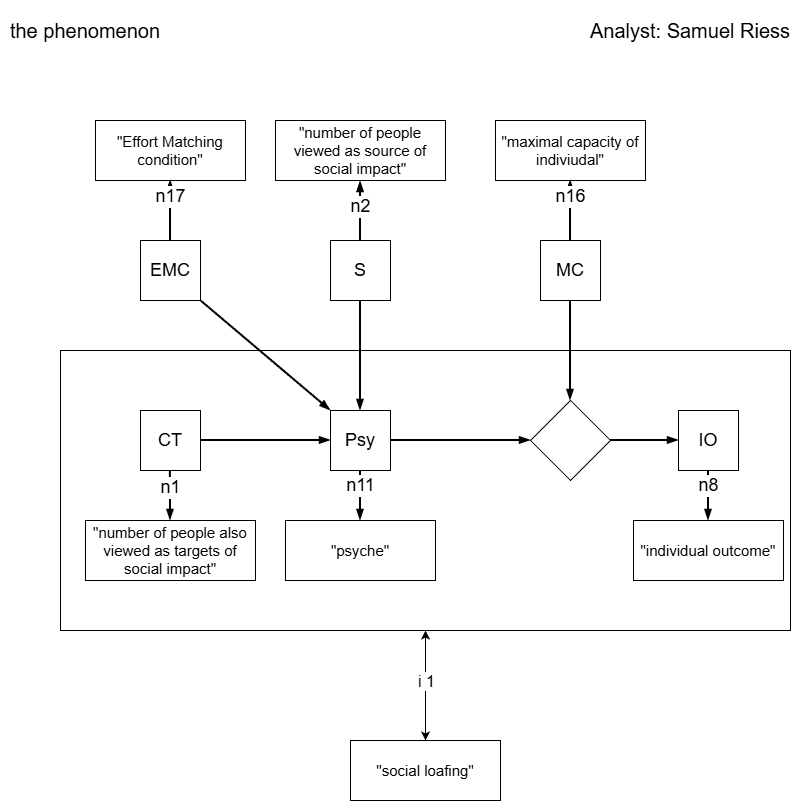
\includegraphics[width=0.8\linewidth,height=\textheight,keepaspectratio]{doc/VAST_SocialLoafing_Phenomenon_image.png}

}

\end{figure}%

To address the robustness of social loafing and therefore the very
reason for investigating it further, we part it into two sections:
Strength of evidence and generalizability, using the UTOS framework. We
get our overview for both sections by analyzing a Meta-Analysis
concerning social loafing (\citeproc{ref-karau1993}{Karau \& Williams,
1993}). We found quotes like ``Both laboratory experiments and field
studies have been conducted using a range of subject populations varying
in age, gender, and culture''. This leads to the assumption that at
least the setting (S) and the Units (U) were varied over the years, for
the meta-analysis conducts about 78 Studies. Others quotes like
``Several studies provided data for more than one relevant dependent
variable'' are leading towards a given generalizability for the
dimension of Outcomes (O) which is additionally supported by quotes like
``used both within- and between-subjects comparisons of individuals'
effort across coactive and collective conditions''. This leads to the
strong assumption that different operationalisations were used whilst
investigating the phenomenon. Further both ``physical or cognitive
effort'' were mentioned as different varieties of operationalisation and
therefore the last dimension of UTOS (T - Treatment) can be considered
fulfilled. The strength of evidence can be acknowledged cause the effect
sizes are estimated using mean effect sizes that ``differed
significantly from the 0.00 value that indicates exactly no
difference''. The most pithy evidence can be found in the result
section. Directly, the mean effect size was found to be d = .44 which
was statistically significant (p \textless{} .001), presenting a
moderate effect according to Cohen's general conventions. Taken
together, the phenomenon can be considered robust because the whole UTOS
framework and the strength of evidence are supported with empirical
data.

\section{Method}\label{method}

All documents used in the process of writing this report can be found
and downloaded through the GitHub repository:
https://github.com/SamRiess/SocialLoafing\_FINAL.git This report refers
to version number v1.0.0. See the .cff file for further information.

\subsection{used software}\label{used-software}

Throughout our formalization, we use the Visual Argument Structure Tool
(VAST, (\citeproc{ref-leising2023}{Leising et al., 2023})) to build a
graphic visualization of the theory and resulting mechanisms. With this
methodology, we are able to define relationships, our understanding of
core constructs and the mechanisms that take place in the process of
social loafing and effort matching. For the computation of our simulated
Data, we used R(hier Versionsnummer einfügen). Our graphic
representation of the formalized theory was enabled throughout the
application draw.io in which we created our VAST model.

\subsection{Formalization of the
(Proto-)Theory}\label{formalization-of-the-proto-theory}

We used the VAST (Visual Argument Structure Tool) as a graphic form of
formalization for our theory. Further information about the VAST and its
application can be found in Leising et al.
(\citeproc{ref-leising2023}{2023}). In the process, it was crucial to
limit our scope, referring to both theory and phenomenon. The main goal
should be understandability, not the whole integrity of the full theory.
We were limiting our scope to the following aspects: we set the
identifiability of the individual effort to non-existent. This can be
justified for that the identifiability wasn't part of the experiments
for social loafing (\citeproc{ref-latanuxe91979}{Latané et al., 1979}),
neither was it for effort matching (\citeproc{ref-jackson1985}{Jackson
\& Harkins, 1985}). Further, we ignore the mentioned multiplicative
connection between immediacy, strength and number of Co-Targets or
Sources (\citeproc{ref-latanuxe91981}{Latané, 1981}). These weren't,
again, part of previous research so we didn't focus on that specific
part of social impact theory. A few more additional assumptions were
crucial for our finalized theory and model to work. Lastly, other
mentioned constructs like the default expectation for other peoples
loafing wasn't specifically evaluated and included. We ought to deal
with this in using the mechanism in the Psy box to generate this default
expectation, tho it wasn't defined directly. With this approach, the
underlying process gains more understandability while the high and low
Effort condition could be included into the Superfunction for our psyche
process without complicating the model itself. the extension of the
maximum capacity was necessary for simulation purposes, it isn't
mentioned in the theory itself. Without implementing this construct, we
weren't able to compute a manifest Variable cause the main output of the
psychological process is just a percentage number which cannot be
measured without a baseline which presents 100\% of the possible effort.
See (Variable Table) for further values. As we're introducing later in
this report, these restrictions or extensions weren't loss-making for
our Model and replication of the loafing effect and therefore providing
a post-hoc evaluation. Our resulting prototype theory which ought to
explain the phenomenon is presented in (Figure~\ref{fig-mechanism}). The
``relationships'' section shows each relationship and its justification,
based on quotes from previous research (labeled with a ``q'' in
TabelleRelationship) or our own assumptions or restrictions. In keeping
this section short, I am mixing up the explanation of the model with its
justification of the described relationships.

\begin{figure}

\caption{\label{fig-mechanism}Structure of the VAST theory and
mechanism}

\centering{

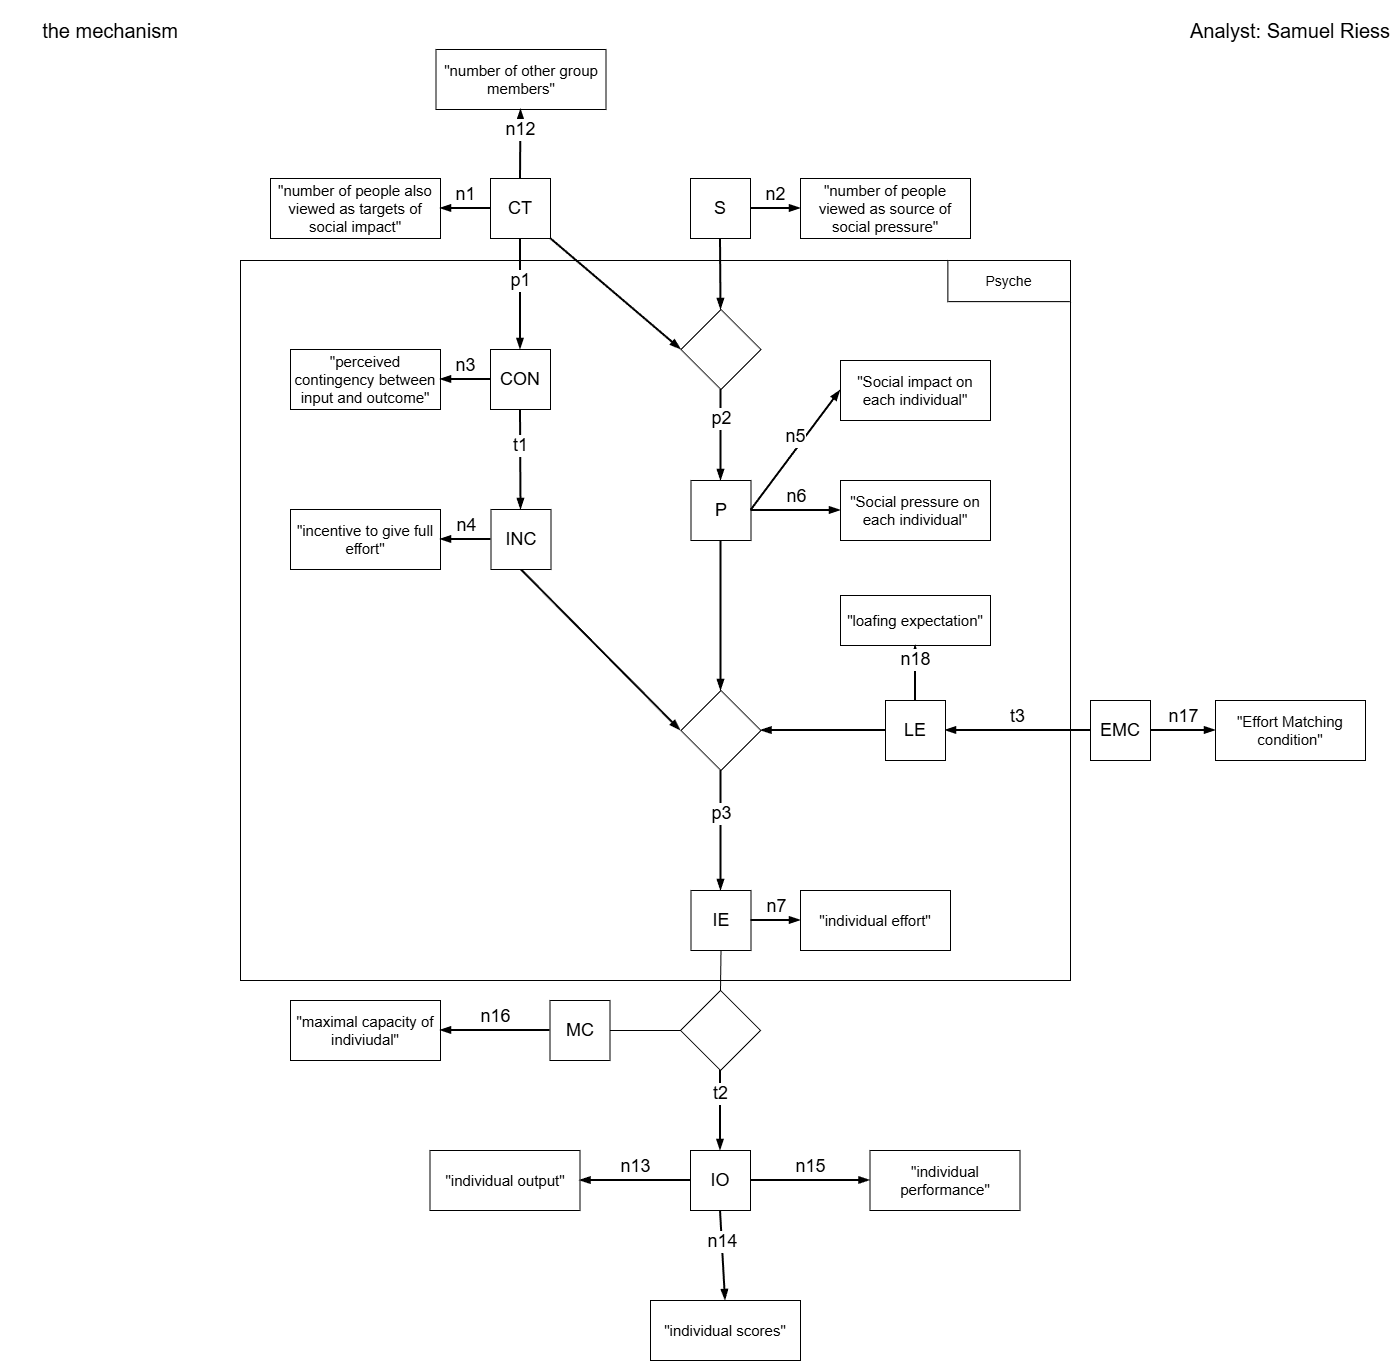
\includegraphics[width=1\linewidth,height=\textheight,keepaspectratio]{doc/VAST_SocialLoafing_Mechanism_Fallacy_image.png}

}

\end{figure}%

\subsubsection{Variables}\label{variables}

All our used variables for each of the constructs, if shown in our VAST,
can be seen in (Tabelle einfügen).

\subsubsection{Relationships}\label{relationships}

All relationships are mentioned in (Tabelle einfügen) which the relevant
quotes, labeled with a ``q'' in the following section. The relationship
between the Co-Targets, Sources and the Pressure on the subject is
presented in Figure~\ref{fig-p2}. We aimed to write a function that is
consistent with exact citations from the sources. Originally, the
pressure can be lowered throughout the number of Co-Targets and Sources
simultaneously. As we can see in the Graphs, the higher the Number of
Sources is, the higher gets the felt impact on one subject. This
represents the classic increase which is mentioned in q4. But with an
increase of the number of Co-Targets, the impact lowered rapidly.
Therefore, consistent with the general interpretation of social impact
theory, felt impact is divided up among the group members (q5-q8).

\begin{figure}

\caption{\label{fig-p2}Plot for the relationsship p2}

\centering{

\pandocbounded{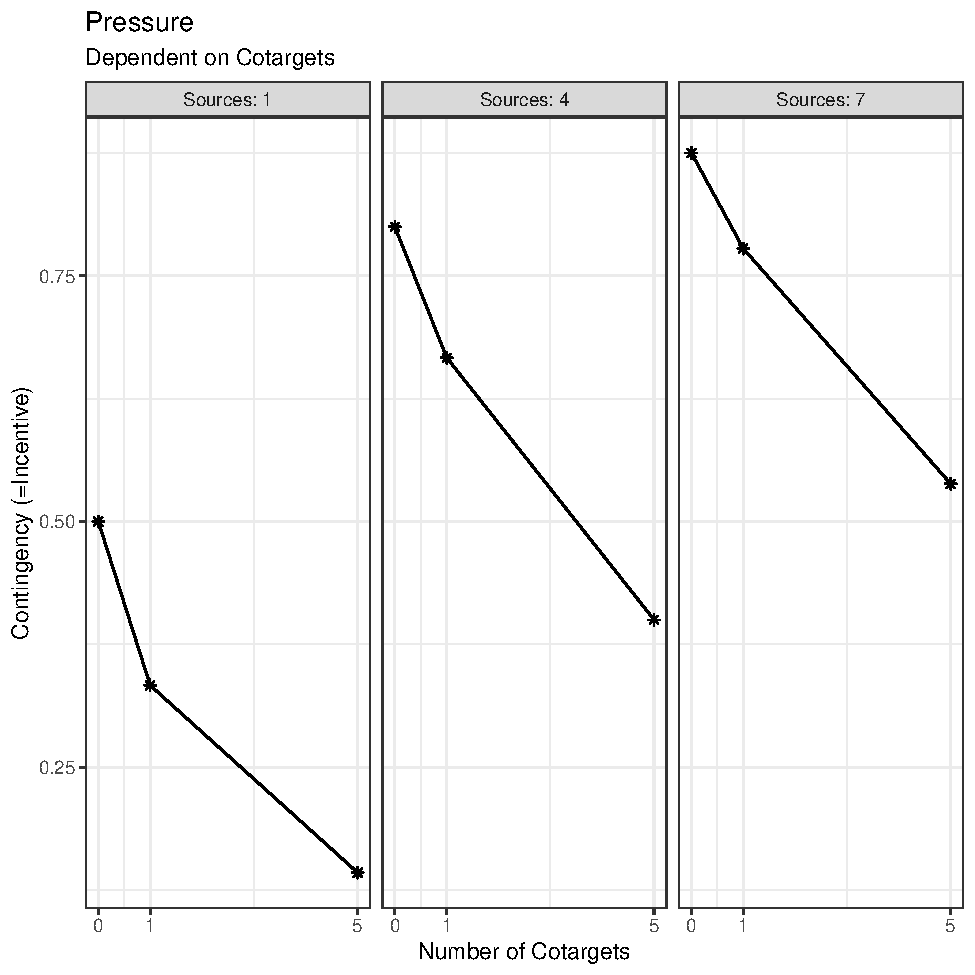
\includegraphics[keepaspectratio]{Report_final_files/figure-pdf/fig-p2-1.pdf}}

}

\end{figure}%

The left path of our VAST (Figure~\ref{fig-mechanism}) is our main
mechanism which produces the phenomenon. It starts with the relationship
between Co-Targets and the contingency which was rather intuitive due to
the specific function derived from the core report, verified with
(\citeproc{ref-latanuxe91979}{Latané et al., 1979}) and specifically in
q1-q3. It is presented in Figure~\ref{fig-p1}.

\begin{figure}

\caption{\label{fig-p1}Plot for the relationsship p1}

\centering{

\pandocbounded{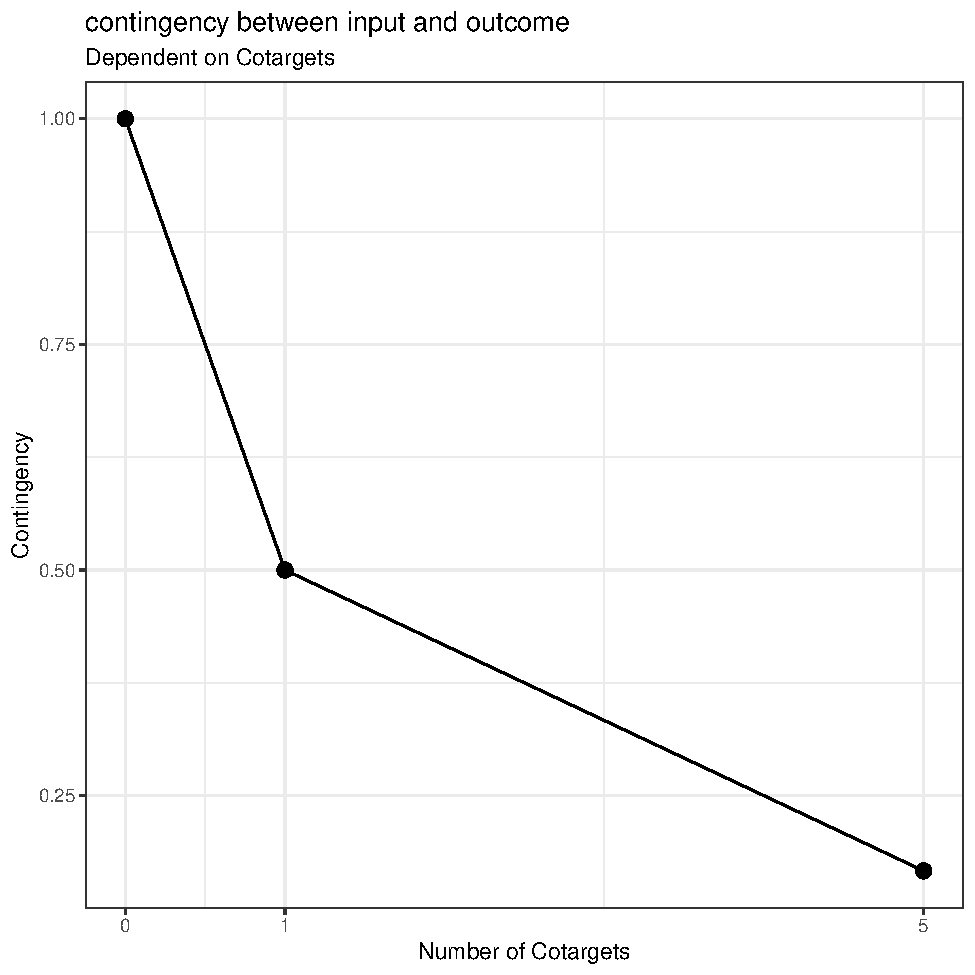
\includegraphics[keepaspectratio]{Report_final_files/figure-pdf/fig-p1-1.pdf}}

}

\end{figure}%

After that, the transformation for the Incentive can be represented by a
proportional increase: Incentive gets the same values as the previously
computed contingency (Figure~\ref{fig-t1}). This was not based on a
focal theory, but we deviated that an incentive to give one's own full
effort directly results from the depicted contingency, also proved with
q14.

\begin{figure}

\caption{\label{fig-t1}Plot for the transformation t1}

\centering{

\pandocbounded{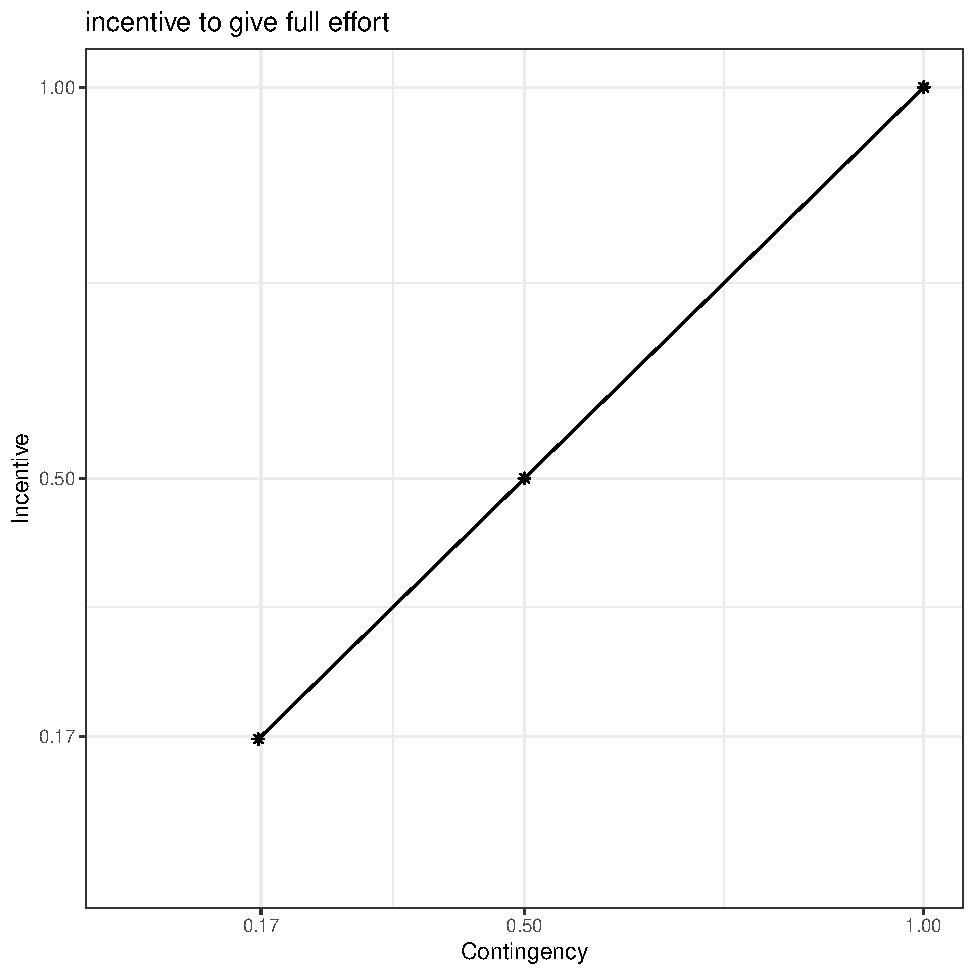
\includegraphics[keepaspectratio]{Report_final_files/figure-pdf/fig-t1-1.pdf}}

}

\end{figure}%

Things were getting more interesting with the function that computes the
resulting individual effort, using all previously computed and simulated
input variables. Both paths of our own VAST meet together in this
relationship. The plot can be viewed in Figure~\ref{fig-p3}, showing the
first influence of our effort Matching condition as well. I wrote a
function which transforms the manifest effort-matching condition (EMC)
into the latent construct of a loafing expectation (LE), named t3 and
supported by q12/q13. If the subject takes action in the LE (low effort)
or HE (high effort) condition, effort matching takes place and fixes
individual effort to a previously fixed value for each condition. These
two values for effort matching conditions can be chosen individually,
but we made sure that its higher in the HE condition compared to the LE
one. The blue graph shows the natural social loafing mechanism for the
individual effort, based on no information whatsoever about the others
effort. First, if the pressure is high, the function starts higher cause
the subject feels more bound to the outcome. Secondly, with more
incentive to give full effort the subject is getting higher values in
the effort. We argue that, besides great pressure, the effort won't
reach its maximum if the incentive to give full effort isn't maximized.
The basic idea of the relationship is supported by q9-q11. We had to
adjust the function to fit in our theory and model so P and IE had a
range from 0-1.

\begin{figure}

\caption{\label{fig-p3}Plot for the relationship p3}

\centering{

\pandocbounded{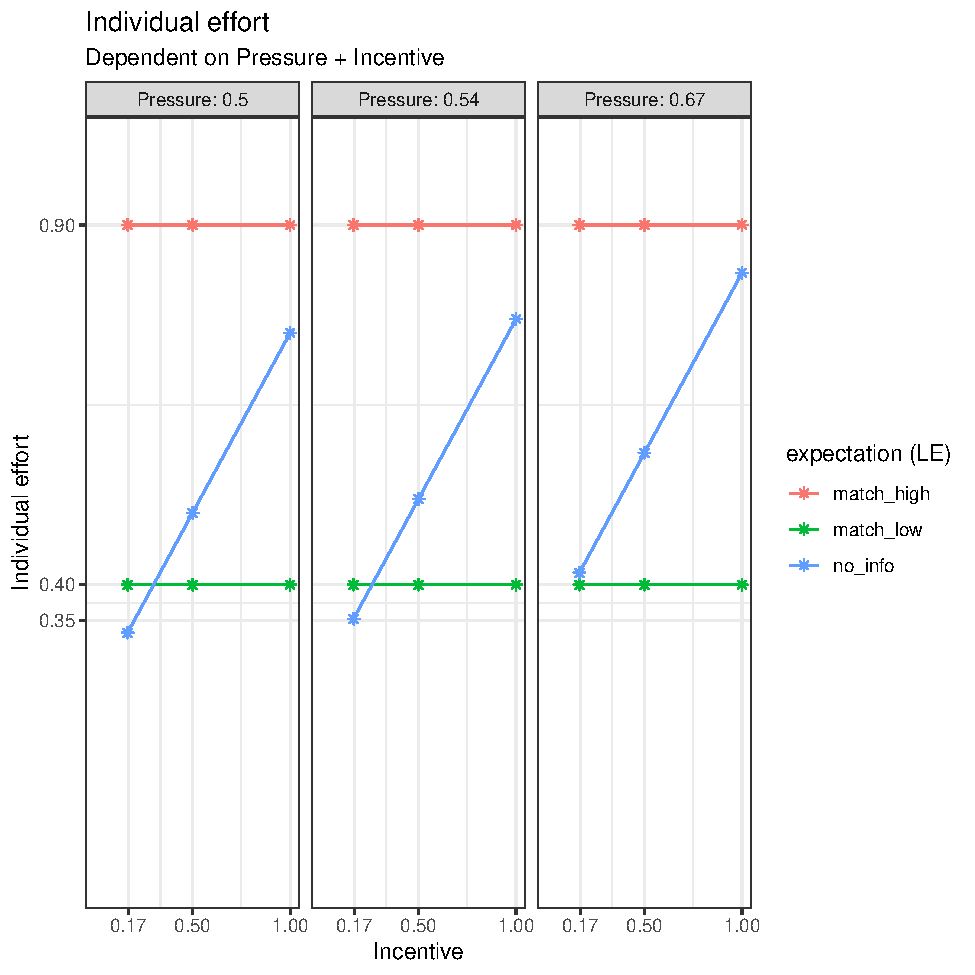
\includegraphics[keepaspectratio]{Report_final_files/figure-pdf/fig-p3-1.pdf}}

}

\end{figure}%

The simulation-relevant relationship we have to show is the
transformation of IE and MC into the individual Output (IO). As can be
seen in Figure~\ref{fig-t2}, the more maximum capacity each subject has,
the higher the value for the outcome is. That occurs because we defined
IE as a percentage of 1 (e.g.~0.6 = 60\%) which is offset against the
maximum. Hence, with more effort, the outcome is increasing
simultaneously. We concluded a interaction effect between MC and IE that
accounts for the final value of one's own output. The transformation
function was needed to compute the manifest outcome for each person
(e.g.~in q15) and the group means for our statistical analysis later on.

\begin{figure}

\caption{\label{fig-t2}Plot for the relationship t2}

\centering{

\pandocbounded{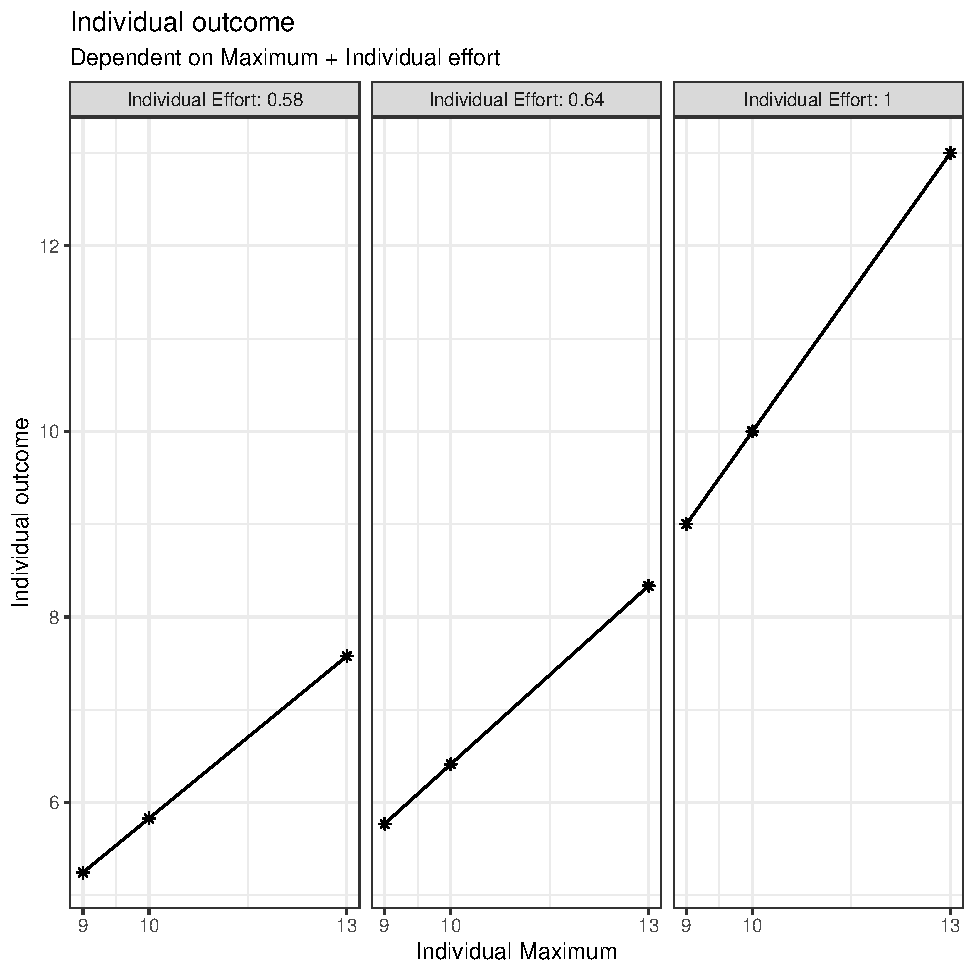
\includegraphics[keepaspectratio]{Report_final_files/figure-pdf/fig-t2-1.pdf}}

}

\end{figure}%

The behavior of the combined system is shown in (). It is pretty similar
to the IE function but deviates in its own input variables. In this
case, we used all manifest ones and threw them into the whole
psychological process that it labeled ``Psyche'' (see
Figure~\ref{fig-vast} for clarification). The resulting
``superfunction'' can be described as followed:

\subsection{Evaluation of the formal
model}\label{evaluation-of-the-formal-model}

Finally, we got to test our model with our simulation. We simulated the
original experiment for social loafing, using the sound pressure as the
individual outcome (\citeproc{ref-latane1979}{\textbf{latane1979?}}) but
added the EMC predictor, known in our theory by ``Effort matching
condition''. With a sample size of n=36 (view
(\citeproc{ref-latane1979}{\textbf{latane1979?}}), we were able to test
for the original effect and the effort matching mechanism in one
sample). The descriptives for both analyses are showcased in
Figure~\ref{fig-box1} and Figure~\ref{fig-box2}. These are highly
influenced by the noise term of p3 and can be adjusted freely. We chose
the parameters mean = 0 and sdd = 0.3 for our ``noise term'' of that
function, cause we assume that variability comes into the model
throughout many sources: e.g.~fatigue, personality, or the current
mental state.

\begin{figure}

\caption{\label{fig-box1}Boxplot for the replication of Latané}

\centering{

\pandocbounded{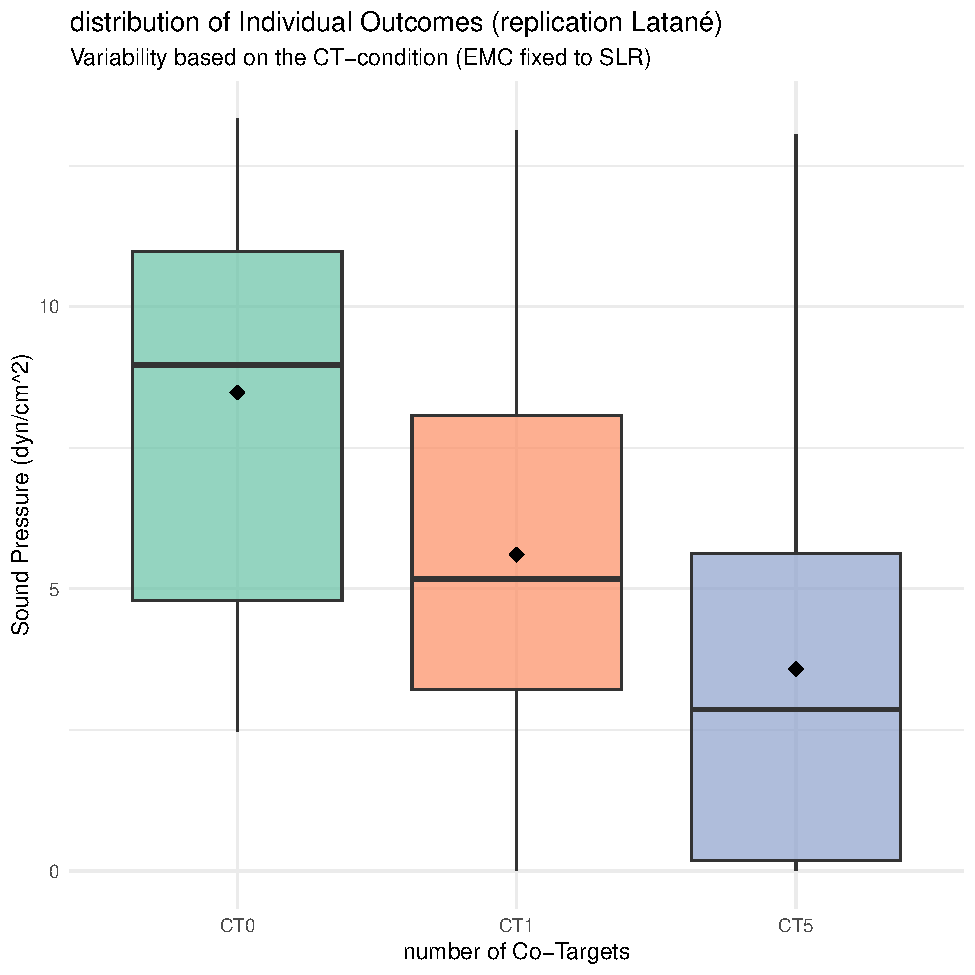
\includegraphics[keepaspectratio]{Report_final_files/figure-pdf/fig-box1-1.pdf}}

}

\end{figure}%

\begin{figure}

\caption{\label{fig-box2}Boxplot for the replication of Jackson \&
Harkins}

\centering{

\pandocbounded{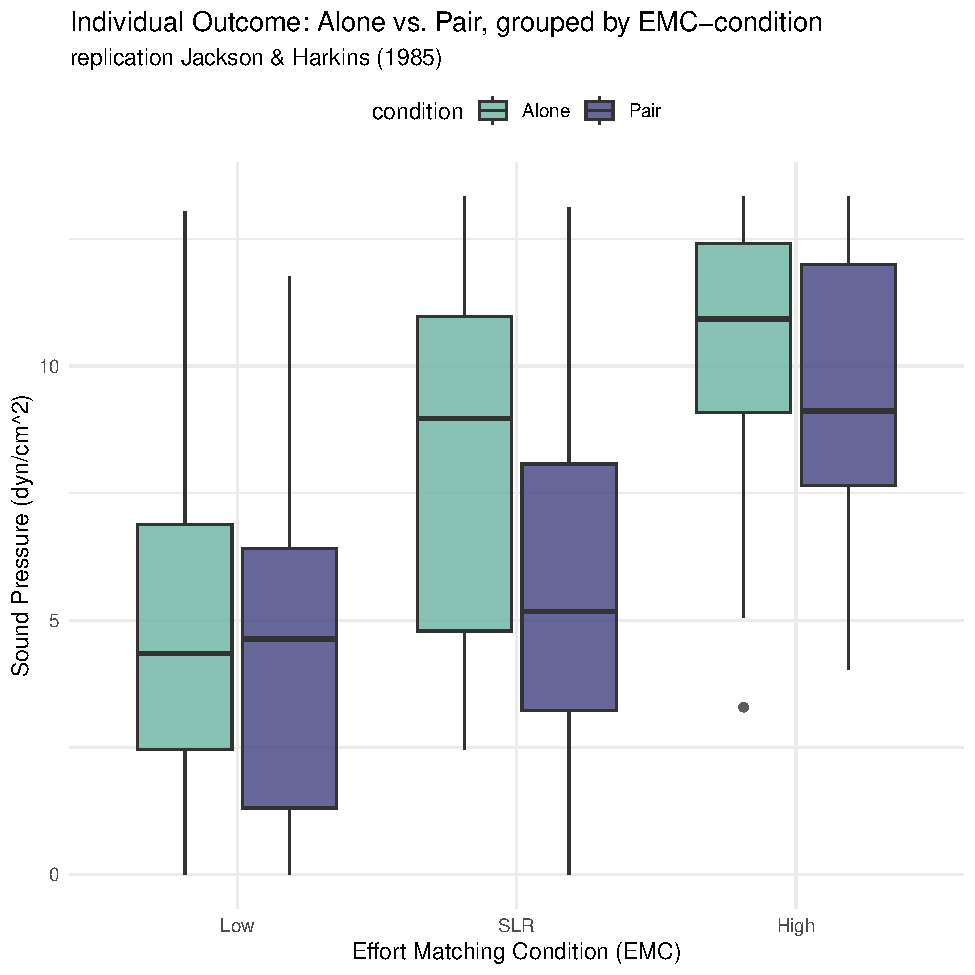
\includegraphics[keepaspectratio]{Report_final_files/figure-pdf/fig-box2-1.pdf}}

}

\end{figure}%

Due to our 2 computed ANOVAS which rely on the same sample, we needed to
adjust our p-value with the Bonferroni method. Thus, the new
\(\alpha\)-niveau is divided by 2 and comes down to .025. It turns out
that both effects, on one side the social loafing but on the other the
elimination of this phenomenon throughout implementing a low and high
Effort condition were supported by our present simulation and therefore
our model. In proving the results, we fall back on the original analysis
(\citeproc{ref-latanuxe91979}{Latané et al., 1979}) for which all
resulting graphs can be viewed in Figure~\ref{fig-final}. The main
replication was significant for the number of Co-Targets had a
significant effect on the individual sound output \(F(2, 105) = 18.56\),
\(\mathit{MSE} = 11.78\), \(p < .001\), \(\hat{\eta}^2_G = .261\). This
is consistent with the findings of (\citeproc{ref-latanuxe91979}{Latané
et al., 1979}) and proves that our model is capable of producing the
main phenomenon. Whilst replicating the findings of effort matching
(\citeproc{ref-jackson1985}{Jackson \& Harkins, 1985}), we compared alle
three Pairs of ``Alone vs.~Group'', each for one condition of EMC. Only
in the SLR-condition, we detected a significant decrease in the outcome
between the group and alone situation (p \textless{} .001). For the low
effort condition the difference was no longer significant with p=.372,
equal results appeared in the the high effort condition with p=.175.
Therefore, we've shown that Effort Matching emerged via our model and is
consistent with the literature in eliminating the social loafing effect
thoroughly holding the loafing expectation constant.

\begin{figure}

\caption{\label{fig-final}Final plot of the simulation}

\centering{

\pandocbounded{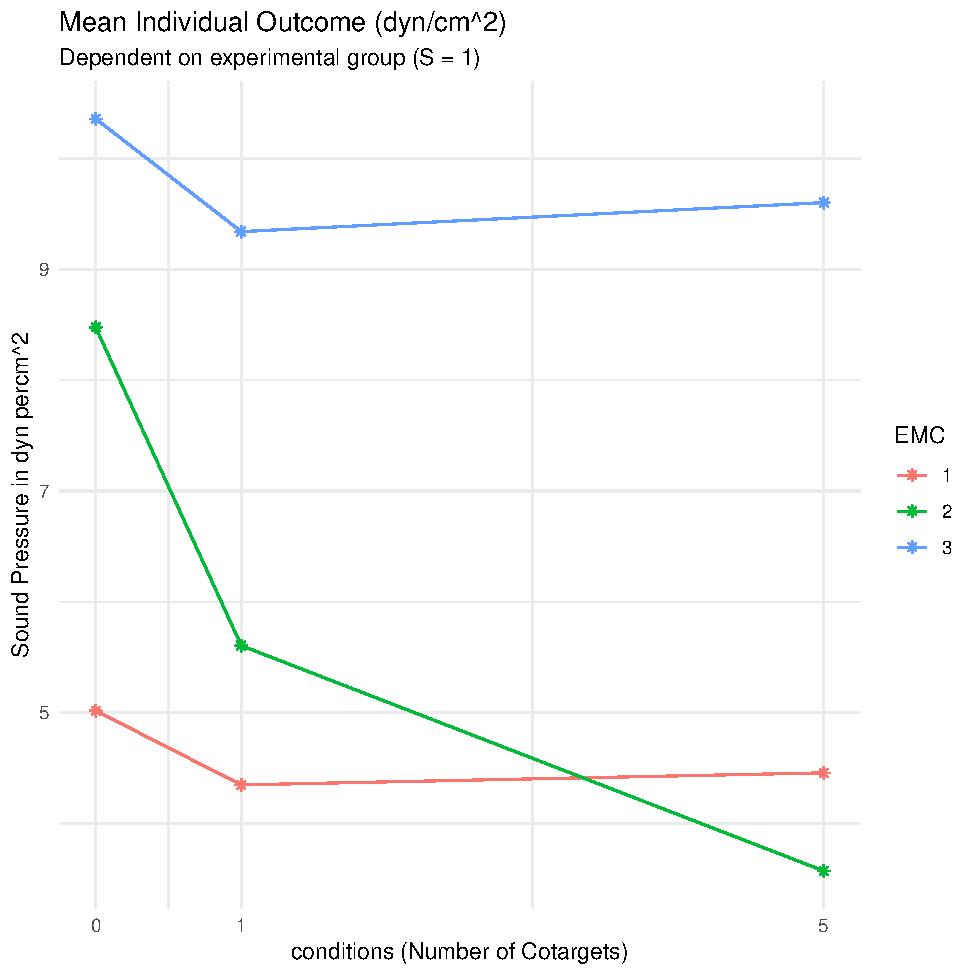
\includegraphics[keepaspectratio]{Report_final_files/figure-pdf/fig-final-1.pdf}}

}

\end{figure}%

\section{Meta-reflection}\label{meta-reflection}

Some issues need to be discussed at the end. First, they original paper
contained many jangle-fallacies, so it was quite difficult to form clear
definitions for our main constructs. An alternative VAST image
(Figure~\ref{fig-vast-nof}) illustrates this conceptual separation,
highlighting that each construct should be clearly defined without
redundant or overlapping terminology. Second, it was a challenge to
implement the sources (S) into our model, as these factors were
conceptualized in the underlying theory but not explicitly manipulated
within the experimental design (\citeproc{ref-latanuxe91979}{Latané et
al., 1979}). A good limitation of the scope was downright necessary in
formalizing this theory while using VAST. Hence, the mentioned
inconsistencies in the original experiment and its explanation had to be
managed. In regard of the simulation, the decision if the VAST itself
was to contain a group level was partially difficult - in the end we
decided to stick with the individual output as the final construct. For
using a group level directly in the VAST we had to adjust the
simulation, the Co-Target construct to ``group members'' and therefore
the whole psychological mechanism of social loafing.

\begin{figure}

\caption{\label{fig-vast-nof}Structure of the loafing mechanism without
Fallacies}

\centering{

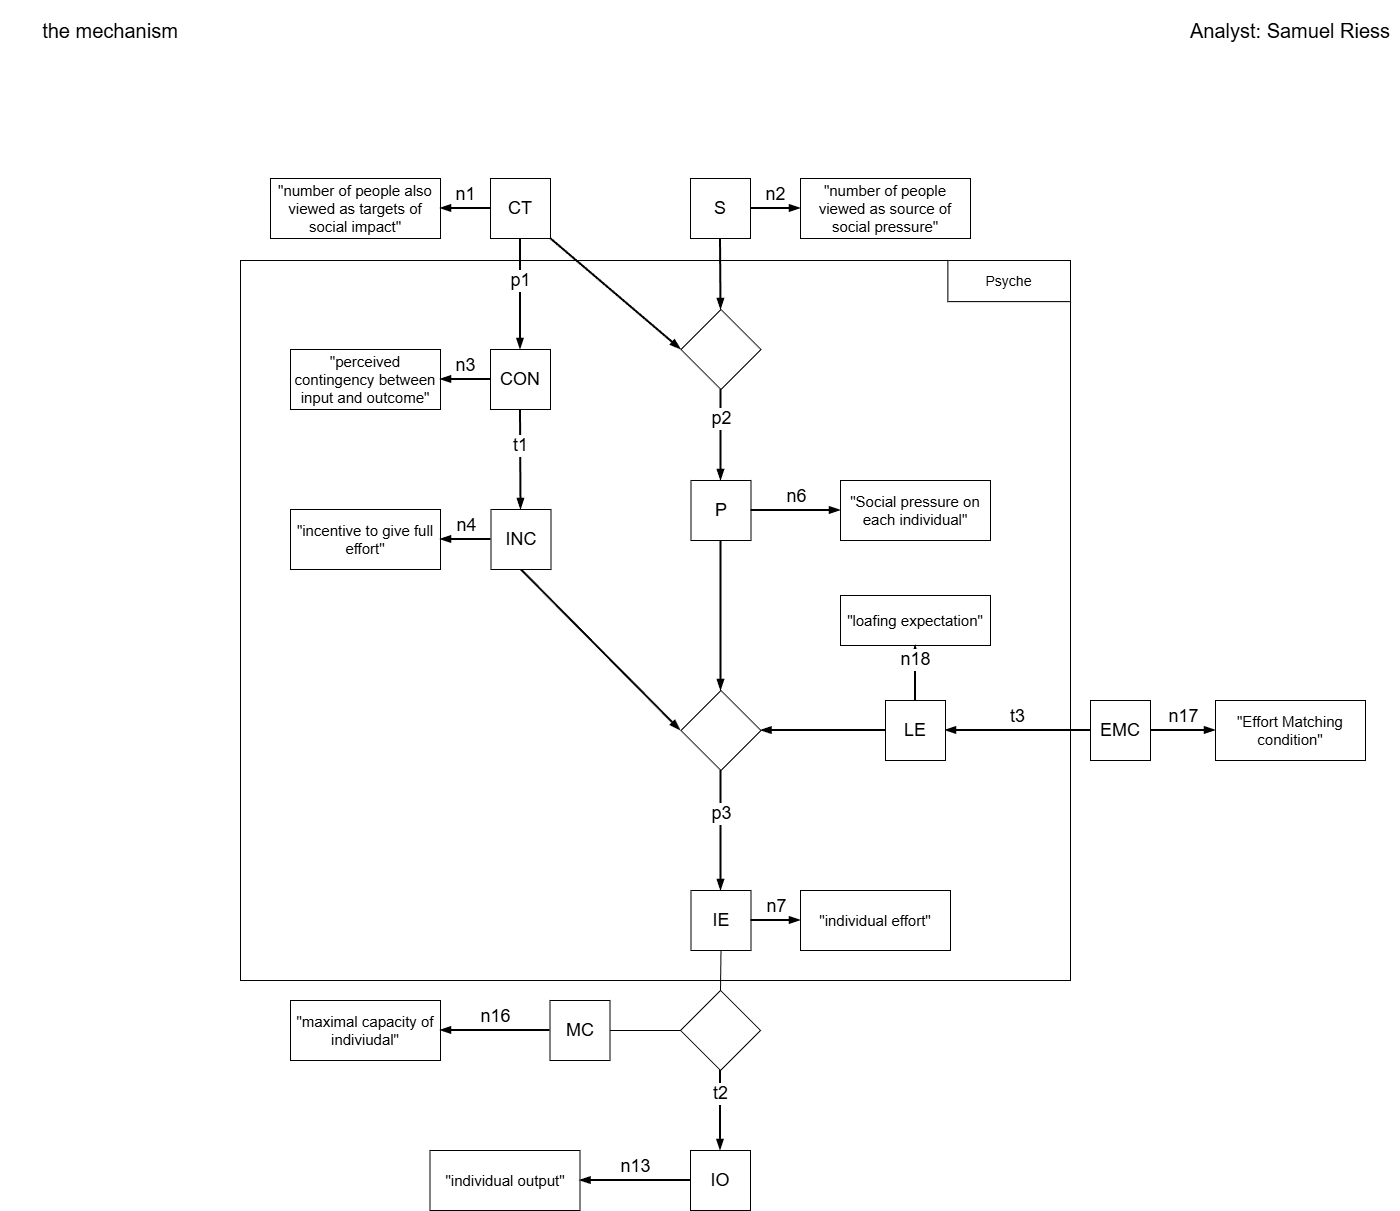
\includegraphics[width=1\linewidth,height=\textheight,keepaspectratio]{doc/VAST_SocialLoafing_Mechanism_noFallacy_image.png}

}

\end{figure}%

\section{References}\label{references}

\phantomsection\label{refs}
\begin{CSLReferences}{1}{0}
\bibitem[\citeproctext]{ref-borsboom2021}
Borsboom, D., Van Der Maas, H. L. J., Dalege, J., Kievit, R. A., \&
Haig, B. D. (2021). Theory Construction Methodology: A Practical
Framework for Building Theories in Psychology. \emph{Perspectives on
Psychological Science}, \emph{16}(4), 756--766.
\url{https://doi.org/10.1177/1745691620969647}

\bibitem[\citeproctext]{ref-jackson1985}
Jackson, J. M., \& Harkins, S. G. (1985). Equity in effort: An
explanation of the social loafing effect. \emph{Journal of Personality
and Social Psychology}, \emph{49}(5), 1199--1206.
\url{https://doi.org/10.1037/0022-3514.49.5.1199}

\bibitem[\citeproctext]{ref-karau1993}
Karau, S. J., \& Williams, K. D. (1993). Social loafing: A meta-analytic
review and theoretical integration. \emph{Journal of Personality and
Social Psychology}, \emph{65}(4), 681--706.
\url{https://doi.org/10.1037/0022-3514.65.4.681}

\bibitem[\citeproctext]{ref-latanuxe91981}
Latané, B. (1981). The psychology of social impact. \emph{American
Psychologist}, \emph{36}(4), 343--356.
\url{https://doi.org/10.1037/0003-066X.36.4.343}

\bibitem[\citeproctext]{ref-latanuxe91979}
Latané, B., Williams, K., \& Harkins, S. (1979). Many hands make light
the work: The causes and consequences of social loafing. \emph{Journal
of Personality and Social Psychology}, \emph{37}(6), 822--832.
\url{https://doi.org/10.1037/0022-3514.37.6.822}

\bibitem[\citeproctext]{ref-leising2023}
Leising, D., Grenke, O., \& Cramer, M. (2023). Visual argument structure
tool (VAST) version 1.0. \emph{Meta-Psychology}, \emph{7}.
\url{https://doi.org/10.15626/MP.2021.2911}

\end{CSLReferences}

\newpage
\appendix

\appendix

\section{}\label{}

\section{}\label{apx-appendix}

\begin{table}

{\caption{{Overview of constructs and
definitions}{\label{tbl-constructs}}}
\vspace{-20pt}}

\global\setlength{\Oldarrayrulewidth}{\arrayrulewidth}

\global\setlength{\Oldtabcolsep}{\tabcolsep}

\setlength{\tabcolsep}{2pt}

\renewcommand*{\arraystretch}{1.5}



\providecommand{\ascline}[3]{\noalign{\global\arrayrulewidth #1}\arrayrulecolor[HTML]{#2}\cline{#3}}

\begin{longtable*}[c]{|p{0.39in}|p{0.79in}|p{1.38in}|p{3.74in}|p{0.75in}|p{0.75in}|p{0.75in}|p{0.75in}}



\ascline{1.5pt}{666666}{1-8}

\multicolumn{1}{>{\raggedright}p{\dimexpr 0.39in+0\tabcolsep}}{\textcolor[HTML]{000000}{\fontsize{9}{9}\selectfont{\global\setmainfont{Arial}{ID}}}} & \multicolumn{1}{>{\raggedright}p{\dimexpr 0.79in+0\tabcolsep}}{\textcolor[HTML]{000000}{\fontsize{9}{9}\selectfont{\global\setmainfont{Arial}{Type}}}} & \multicolumn{1}{>{\raggedright}p{\dimexpr 1.38in+0\tabcolsep}}{\textcolor[HTML]{000000}{\fontsize{9}{9}\selectfont{\global\setmainfont{Arial}{Short\ name}}}} & \multicolumn{1}{>{\raggedright}p{\dimexpr 3.74in+0\tabcolsep}}{\textcolor[HTML]{000000}{\fontsize{9}{9}\selectfont{\global\setmainfont{Arial}{Quote}}}} & \multicolumn{1}{>{\raggedright}p{\dimexpr 0.75in+0\tabcolsep}}{\textcolor[HTML]{000000}{\fontsize{9}{9}\selectfont{\global\setmainfont{Arial}{Reference}}}} & \multicolumn{1}{>{\raggedright}p{\dimexpr 0.75in+0\tabcolsep}}{\textcolor[HTML]{000000}{\fontsize{9}{9}\selectfont{\global\setmainfont{Arial}{Rel.\ type\ (n,\ p,\ i,\ r,\ ...)}}}} & \multicolumn{1}{>{\raggedright}p{\dimexpr 0.75in+0\tabcolsep}}{\textcolor[HTML]{000000}{\fontsize{9}{9}\selectfont{\global\setmainfont{Arial}{Comment\ (e.g.,\ identified\ gaps\ \&\ inconsistencies)}}}} & \multicolumn{1}{>{\raggedright}p{\dimexpr 0.75in+0\tabcolsep}}{\textcolor[HTML]{000000}{\fontsize{9}{9}\selectfont{\global\setmainfont{Arial}{Incl.\ (Y/N)?}}}} \\

\ascline{1.5pt}{666666}{1-8}\endfirsthead 

\ascline{1.5pt}{666666}{1-8}

\multicolumn{1}{>{\raggedright}p{\dimexpr 0.39in+0\tabcolsep}}{\textcolor[HTML]{000000}{\fontsize{9}{9}\selectfont{\global\setmainfont{Arial}{ID}}}} & \multicolumn{1}{>{\raggedright}p{\dimexpr 0.79in+0\tabcolsep}}{\textcolor[HTML]{000000}{\fontsize{9}{9}\selectfont{\global\setmainfont{Arial}{Type}}}} & \multicolumn{1}{>{\raggedright}p{\dimexpr 1.38in+0\tabcolsep}}{\textcolor[HTML]{000000}{\fontsize{9}{9}\selectfont{\global\setmainfont{Arial}{Short\ name}}}} & \multicolumn{1}{>{\raggedright}p{\dimexpr 3.74in+0\tabcolsep}}{\textcolor[HTML]{000000}{\fontsize{9}{9}\selectfont{\global\setmainfont{Arial}{Quote}}}} & \multicolumn{1}{>{\raggedright}p{\dimexpr 0.75in+0\tabcolsep}}{\textcolor[HTML]{000000}{\fontsize{9}{9}\selectfont{\global\setmainfont{Arial}{Reference}}}} & \multicolumn{1}{>{\raggedright}p{\dimexpr 0.75in+0\tabcolsep}}{\textcolor[HTML]{000000}{\fontsize{9}{9}\selectfont{\global\setmainfont{Arial}{Rel.\ type\ (n,\ p,\ i,\ r,\ ...)}}}} & \multicolumn{1}{>{\raggedright}p{\dimexpr 0.75in+0\tabcolsep}}{\textcolor[HTML]{000000}{\fontsize{9}{9}\selectfont{\global\setmainfont{Arial}{Comment\ (e.g.,\ identified\ gaps\ \&\ inconsistencies)}}}} & \multicolumn{1}{>{\raggedright}p{\dimexpr 0.75in+0\tabcolsep}}{\textcolor[HTML]{000000}{\fontsize{9}{9}\selectfont{\global\setmainfont{Arial}{Incl.\ (Y/N)?}}}} \\

\ascline{1.5pt}{666666}{1-8}\endhead



\multicolumn{1}{>{\raggedright}p{\dimexpr 0.39in+0\tabcolsep}}{\textcolor[HTML]{000000}{\fontsize{9}{9}\selectfont{\global\setmainfont{Arial}{}}}} & \multicolumn{1}{>{\raggedright}p{\dimexpr 0.79in+0\tabcolsep}}{\textcolor[HTML]{000000}{\fontsize{9}{9}\selectfont{\global\setmainfont{Arial}{-\ Phenomenon}}}} & \multicolumn{1}{>{\raggedright}p{\dimexpr 1.38in+0\tabcolsep}}{\textcolor[HTML]{000000}{\fontsize{9}{9}\selectfont{\global\setmainfont{Arial}{}}}} & \multicolumn{1}{>{\raggedright}p{\dimexpr 3.74in+0\tabcolsep}}{\textcolor[HTML]{000000}{\fontsize{9}{9}\selectfont{\global\setmainfont{Arial}{}}}} & \multicolumn{1}{>{\raggedright}p{\dimexpr 0.75in+0\tabcolsep}}{\textcolor[HTML]{000000}{\fontsize{9}{9}\selectfont{\global\setmainfont{Arial}{}}}} & \multicolumn{1}{>{\raggedright}p{\dimexpr 0.75in+0\tabcolsep}}{\textcolor[HTML]{000000}{\fontsize{9}{9}\selectfont{\global\setmainfont{Arial}{}}}} & \multicolumn{1}{>{\raggedright}p{\dimexpr 0.75in+0\tabcolsep}}{\textcolor[HTML]{000000}{\fontsize{9}{9}\selectfont{\global\setmainfont{Arial}{}}}} & \multicolumn{1}{>{\raggedright}p{\dimexpr 0.75in+0\tabcolsep}}{\textcolor[HTML]{000000}{\fontsize{9}{9}\selectfont{\global\setmainfont{Arial}{}}}} \\





\multicolumn{1}{>{\raggedright}p{\dimexpr 0.39in+0\tabcolsep}}{\textcolor[HTML]{000000}{\fontsize{9}{9}\selectfont{\global\setmainfont{Arial}{}}}} & \multicolumn{1}{>{\raggedright}p{\dimexpr 0.79in+0\tabcolsep}}{\textcolor[HTML]{000000}{\fontsize{9}{9}\selectfont{\global\setmainfont{Arial}{-\ Concept}}}} & \multicolumn{1}{>{\raggedright}p{\dimexpr 1.38in+0\tabcolsep}}{\textcolor[HTML]{000000}{\fontsize{9}{9}\selectfont{\global\setmainfont{Arial}{}}}} & \multicolumn{1}{>{\raggedright}p{\dimexpr 3.74in+0\tabcolsep}}{\textcolor[HTML]{000000}{\fontsize{9}{9}\selectfont{\global\setmainfont{Arial}{}}}} & \multicolumn{1}{>{\raggedright}p{\dimexpr 0.75in+0\tabcolsep}}{\textcolor[HTML]{000000}{\fontsize{9}{9}\selectfont{\global\setmainfont{Arial}{}}}} & \multicolumn{1}{>{\raggedright}p{\dimexpr 0.75in+0\tabcolsep}}{\textcolor[HTML]{000000}{\fontsize{9}{9}\selectfont{\global\setmainfont{Arial}{}}}} & \multicolumn{1}{>{\raggedright}p{\dimexpr 0.75in+0\tabcolsep}}{\textcolor[HTML]{000000}{\fontsize{9}{9}\selectfont{\global\setmainfont{Arial}{}}}} & \multicolumn{1}{>{\raggedright}p{\dimexpr 0.75in+0\tabcolsep}}{\textcolor[HTML]{000000}{\fontsize{9}{9}\selectfont{\global\setmainfont{Arial}{}}}} \\





\multicolumn{1}{>{\raggedright}p{\dimexpr 0.39in+0\tabcolsep}}{\textcolor[HTML]{000000}{\fontsize{9}{9}\selectfont{\global\setmainfont{Arial}{}}}} & \multicolumn{1}{>{\raggedright}p{\dimexpr 0.79in+0\tabcolsep}}{\textcolor[HTML]{000000}{\fontsize{9}{9}\selectfont{\global\setmainfont{Arial}{-\ HOC}}}} & \multicolumn{1}{>{\raggedright}p{\dimexpr 1.38in+0\tabcolsep}}{\textcolor[HTML]{000000}{\fontsize{9}{9}\selectfont{\global\setmainfont{Arial}{}}}} & \multicolumn{1}{>{\raggedright}p{\dimexpr 3.74in+0\tabcolsep}}{\textcolor[HTML]{000000}{\fontsize{9}{9}\selectfont{\global\setmainfont{Arial}{}}}} & \multicolumn{1}{>{\raggedright}p{\dimexpr 0.75in+0\tabcolsep}}{\textcolor[HTML]{000000}{\fontsize{9}{9}\selectfont{\global\setmainfont{Arial}{}}}} & \multicolumn{1}{>{\raggedright}p{\dimexpr 0.75in+0\tabcolsep}}{\textcolor[HTML]{000000}{\fontsize{9}{9}\selectfont{\global\setmainfont{Arial}{}}}} & \multicolumn{1}{>{\raggedright}p{\dimexpr 0.75in+0\tabcolsep}}{\textcolor[HTML]{000000}{\fontsize{9}{9}\selectfont{\global\setmainfont{Arial}{}}}} & \multicolumn{1}{>{\raggedright}p{\dimexpr 0.75in+0\tabcolsep}}{\textcolor[HTML]{000000}{\fontsize{9}{9}\selectfont{\global\setmainfont{Arial}{}}}} \\





\multicolumn{1}{>{\raggedright}p{\dimexpr 0.39in+0\tabcolsep}}{\textcolor[HTML]{000000}{\fontsize{9}{9}\selectfont{\global\setmainfont{Arial}{CT }}}} & \multicolumn{1}{>{\raggedright}p{\dimexpr 0.79in+0\tabcolsep}}{\textcolor[HTML]{000000}{\fontsize{9}{9}\selectfont{\global\setmainfont{Arial}{C}}}} & \multicolumn{1}{>{\raggedright}p{\dimexpr 1.38in+0\tabcolsep}}{\textcolor[HTML]{000000}{\fontsize{9}{9}\selectfont{\global\setmainfont{Arial}{Co-Targets}}}} & \multicolumn{1}{>{\raggedright}p{\dimexpr 3.74in+0\tabcolsep}}{\textcolor[HTML]{000000}{\fontsize{9}{9}\selectfont{\global\setmainfont{Arial}{-“The\ more\ people\ who\ are\ the\ target}}}} & \multicolumn{1}{>{\raggedright}p{\dimexpr 0.75in+0\tabcolsep}}{\textcolor[HTML]{000000}{\fontsize{9}{9}\selectfont{\global\setmainfont{Arial}{Latané\ et\ al.,\ S.823\ (1979)}}}} & \multicolumn{1}{>{\raggedright}p{\dimexpr 0.75in+0\tabcolsep}}{\textcolor[HTML]{000000}{\fontsize{9}{9}\selectfont{\global\setmainfont{Arial}{n1,\ p1,p2,\ n12}}}} & \multicolumn{1}{>{\raggedright}p{\dimexpr 0.75in+0\tabcolsep}}{\textcolor[HTML]{000000}{\fontsize{9}{9}\selectfont{\global\setmainfont{Arial}{}}}} & \multicolumn{1}{>{\raggedright}p{\dimexpr 0.75in+0\tabcolsep}}{\textcolor[HTML]{000000}{\fontsize{9}{9}\selectfont{\global\setmainfont{Arial}{Y}}}} \\





\multicolumn{1}{>{\raggedright}p{\dimexpr 0.39in+0\tabcolsep}}{\textcolor[HTML]{000000}{\fontsize{9}{9}\selectfont{\global\setmainfont{Arial}{}}}} & \multicolumn{1}{>{\raggedright}p{\dimexpr 0.79in+0\tabcolsep}}{\textcolor[HTML]{000000}{\fontsize{9}{9}\selectfont{\global\setmainfont{Arial}{}}}} & \multicolumn{1}{>{\raggedright}p{\dimexpr 1.38in+0\tabcolsep}}{\textcolor[HTML]{000000}{\fontsize{9}{9}\selectfont{\global\setmainfont{Arial}{}}}} & \multicolumn{1}{>{\raggedright}p{\dimexpr 3.74in+0\tabcolsep}}{\textcolor[HTML]{000000}{\fontsize{9}{9}\selectfont{\global\setmainfont{Arial}{of\ this\ pressure,\ [...]”\ (S.823)}}}} & \multicolumn{1}{>{\raggedright}p{\dimexpr 0.75in+0\tabcolsep}}{\textcolor[HTML]{000000}{\fontsize{9}{9}\selectfont{\global\setmainfont{Arial}{}}}} & \multicolumn{1}{>{\raggedright}p{\dimexpr 0.75in+0\tabcolsep}}{\textcolor[HTML]{000000}{\fontsize{9}{9}\selectfont{\global\setmainfont{Arial}{}}}} & \multicolumn{1}{>{\raggedright}p{\dimexpr 0.75in+0\tabcolsep}}{\textcolor[HTML]{000000}{\fontsize{9}{9}\selectfont{\global\setmainfont{Arial}{}}}} & \multicolumn{1}{>{\raggedright}p{\dimexpr 0.75in+0\tabcolsep}}{\textcolor[HTML]{000000}{\fontsize{9}{9}\selectfont{\global\setmainfont{Arial}{}}}} \\





\multicolumn{1}{>{\raggedright}p{\dimexpr 0.39in+0\tabcolsep}}{\textcolor[HTML]{000000}{\fontsize{9}{9}\selectfont{\global\setmainfont{Arial}{}}}} & \multicolumn{1}{>{\raggedright}p{\dimexpr 0.79in+0\tabcolsep}}{\textcolor[HTML]{000000}{\fontsize{9}{9}\selectfont{\global\setmainfont{Arial}{}}}} & \multicolumn{1}{>{\raggedright}p{\dimexpr 1.38in+0\tabcolsep}}{\textcolor[HTML]{000000}{\fontsize{9}{9}\selectfont{\global\setmainfont{Arial}{}}}} & \multicolumn{1}{>{\raggedright}p{\dimexpr 3.74in+0\tabcolsep}}{\textcolor[HTML]{000000}{\fontsize{9}{9}\selectfont{\global\setmainfont{Arial}{}}}} & \multicolumn{1}{>{\raggedright}p{\dimexpr 0.75in+0\tabcolsep}}{\textcolor[HTML]{000000}{\fontsize{9}{9}\selectfont{\global\setmainfont{Arial}{AND }}}} & \multicolumn{1}{>{\raggedright}p{\dimexpr 0.75in+0\tabcolsep}}{\textcolor[HTML]{000000}{\fontsize{9}{9}\selectfont{\global\setmainfont{Arial}{}}}} & \multicolumn{1}{>{\raggedright}p{\dimexpr 0.75in+0\tabcolsep}}{\textcolor[HTML]{000000}{\fontsize{9}{9}\selectfont{\global\setmainfont{Arial}{}}}} & \multicolumn{1}{>{\raggedright}p{\dimexpr 0.75in+0\tabcolsep}}{\textcolor[HTML]{000000}{\fontsize{9}{9}\selectfont{\global\setmainfont{Arial}{}}}} \\





\multicolumn{1}{>{\raggedright}p{\dimexpr 0.39in+0\tabcolsep}}{\textcolor[HTML]{000000}{\fontsize{9}{9}\selectfont{\global\setmainfont{Arial}{}}}} & \multicolumn{1}{>{\raggedright}p{\dimexpr 0.79in+0\tabcolsep}}{\textcolor[HTML]{000000}{\fontsize{9}{9}\selectfont{\global\setmainfont{Arial}{}}}} & \multicolumn{1}{>{\raggedright}p{\dimexpr 1.38in+0\tabcolsep}}{\textcolor[HTML]{000000}{\fontsize{9}{9}\selectfont{\global\setmainfont{Arial}{}}}} & \multicolumn{1}{>{\raggedright}p{\dimexpr 3.74in+0\tabcolsep}}{\textcolor[HTML]{000000}{\fontsize{9}{9}\selectfont{\global\setmainfont{Arial}{-\ “According\ to\ Latane's\ (1981)\ social\ impact\ theory,\ people\ can\ be\ viewed\ as\ […]\ targets\ of\ social\ impact.” \ (S.\ 682)}}}} & \multicolumn{1}{>{\raggedright}p{\dimexpr 0.75in+0\tabcolsep}}{\textcolor[HTML]{000000}{\fontsize{9}{9}\selectfont{\global\setmainfont{Arial}{Karau\ \&\ Williams,\ S.\ 682\ (1993)}}}} & \multicolumn{1}{>{\raggedright}p{\dimexpr 0.75in+0\tabcolsep}}{\textcolor[HTML]{000000}{\fontsize{9}{9}\selectfont{\global\setmainfont{Arial}{}}}} & \multicolumn{1}{>{\raggedright}p{\dimexpr 0.75in+0\tabcolsep}}{\textcolor[HTML]{000000}{\fontsize{9}{9}\selectfont{\global\setmainfont{Arial}{}}}} & \multicolumn{1}{>{\raggedright}p{\dimexpr 0.75in+0\tabcolsep}}{\textcolor[HTML]{000000}{\fontsize{9}{9}\selectfont{\global\setmainfont{Arial}{}}}} \\





\multicolumn{1}{>{\raggedright}p{\dimexpr 0.39in+0\tabcolsep}}{\textcolor[HTML]{000000}{\fontsize{9}{9}\selectfont{\global\setmainfont{Arial}{}}}} & \multicolumn{1}{>{\raggedright}p{\dimexpr 0.79in+0\tabcolsep}}{\textcolor[HTML]{000000}{\fontsize{9}{9}\selectfont{\global\setmainfont{Arial}{}}}} & \multicolumn{1}{>{\raggedright}p{\dimexpr 1.38in+0\tabcolsep}}{\textcolor[HTML]{000000}{\fontsize{9}{9}\selectfont{\global\setmainfont{Arial}{}}}} & \multicolumn{1}{>{\raggedright}p{\dimexpr 3.74in+0\tabcolsep}}{\textcolor[HTML]{000000}{\fontsize{9}{9}\selectfont{\global\setmainfont{Arial}{}}}} & \multicolumn{1}{>{\raggedright}p{\dimexpr 0.75in+0\tabcolsep}}{\textcolor[HTML]{000000}{\fontsize{9}{9}\selectfont{\global\setmainfont{Arial}{}}}} & \multicolumn{1}{>{\raggedright}p{\dimexpr 0.75in+0\tabcolsep}}{\textcolor[HTML]{000000}{\fontsize{9}{9}\selectfont{\global\setmainfont{Arial}{}}}} & \multicolumn{1}{>{\raggedright}p{\dimexpr 0.75in+0\tabcolsep}}{\textcolor[HTML]{000000}{\fontsize{9}{9}\selectfont{\global\setmainfont{Arial}{}}}} & \multicolumn{1}{>{\raggedright}p{\dimexpr 0.75in+0\tabcolsep}}{\textcolor[HTML]{000000}{\fontsize{9}{9}\selectfont{\global\setmainfont{Arial}{}}}} \\





\multicolumn{1}{>{\raggedright}p{\dimexpr 0.39in+0\tabcolsep}}{\textcolor[HTML]{000000}{\fontsize{9}{9}\selectfont{\global\setmainfont{Arial}{}}}} & \multicolumn{1}{>{\raggedright}p{\dimexpr 0.79in+0\tabcolsep}}{\textcolor[HTML]{000000}{\fontsize{9}{9}\selectfont{\global\setmainfont{Arial}{}}}} & \multicolumn{1}{>{\raggedright}p{\dimexpr 1.38in+0\tabcolsep}}{\textcolor[HTML]{000000}{\fontsize{9}{9}\selectfont{\global\setmainfont{Arial}{}}}} & \multicolumn{1}{>{\raggedright}p{\dimexpr 3.74in+0\tabcolsep}}{\textcolor[HTML]{000000}{\fontsize{9}{9}\selectfont{\global\setmainfont{Arial}{AND}}}} & \multicolumn{1}{>{\raggedright}p{\dimexpr 0.75in+0\tabcolsep}}{\textcolor[HTML]{000000}{\fontsize{9}{9}\selectfont{\global\setmainfont{Arial}{}}}} & \multicolumn{1}{>{\raggedright}p{\dimexpr 0.75in+0\tabcolsep}}{\textcolor[HTML]{000000}{\fontsize{9}{9}\selectfont{\global\setmainfont{Arial}{}}}} & \multicolumn{1}{>{\raggedright}p{\dimexpr 0.75in+0\tabcolsep}}{\textcolor[HTML]{000000}{\fontsize{9}{9}\selectfont{\global\setmainfont{Arial}{}}}} & \multicolumn{1}{>{\raggedright}p{\dimexpr 0.75in+0\tabcolsep}}{\textcolor[HTML]{000000}{\fontsize{9}{9}\selectfont{\global\setmainfont{Arial}{}}}} \\





\multicolumn{1}{>{\raggedright}p{\dimexpr 0.39in+0\tabcolsep}}{\textcolor[HTML]{000000}{\fontsize{9}{9}\selectfont{\global\setmainfont{Arial}{}}}} & \multicolumn{1}{>{\raggedright}p{\dimexpr 0.79in+0\tabcolsep}}{\textcolor[HTML]{000000}{\fontsize{9}{9}\selectfont{\global\setmainfont{Arial}{}}}} & \multicolumn{1}{>{\raggedright}p{\dimexpr 1.38in+0\tabcolsep}}{\textcolor[HTML]{000000}{\fontsize{9}{9}\selectfont{\global\setmainfont{Arial}{}}}} & \multicolumn{1}{>{\raggedright}p{\dimexpr 3.74in+0\tabcolsep}}{\textcolor[HTML]{000000}{\fontsize{9}{9}\selectfont{\global\setmainfont{Arial}{}}}} & \multicolumn{1}{>{\raggedright}p{\dimexpr 0.75in+0\tabcolsep}}{\textcolor[HTML]{000000}{\fontsize{9}{9}\selectfont{\global\setmainfont{Arial}{}}}} & \multicolumn{1}{>{\raggedright}p{\dimexpr 0.75in+0\tabcolsep}}{\textcolor[HTML]{000000}{\fontsize{9}{9}\selectfont{\global\setmainfont{Arial}{}}}} & \multicolumn{1}{>{\raggedright}p{\dimexpr 0.75in+0\tabcolsep}}{\textcolor[HTML]{000000}{\fontsize{9}{9}\selectfont{\global\setmainfont{Arial}{}}}} & \multicolumn{1}{>{\raggedright}p{\dimexpr 0.75in+0\tabcolsep}}{\textcolor[HTML]{000000}{\fontsize{9}{9}\selectfont{\global\setmainfont{Arial}{}}}} \\





\multicolumn{1}{>{\raggedright}p{\dimexpr 0.39in+0\tabcolsep}}{\textcolor[HTML]{000000}{\fontsize{9}{9}\selectfont{\global\setmainfont{Arial}{}}}} & \multicolumn{1}{>{\raggedright}p{\dimexpr 0.79in+0\tabcolsep}}{\textcolor[HTML]{000000}{\fontsize{9}{9}\selectfont{\global\setmainfont{Arial}{}}}} & \multicolumn{1}{>{\raggedright}p{\dimexpr 1.38in+0\tabcolsep}}{\textcolor[HTML]{000000}{\fontsize{9}{9}\selectfont{\global\setmainfont{Arial}{}}}} & \multicolumn{1}{>{\raggedright}p{\dimexpr 3.74in+0\tabcolsep}}{\textcolor[HTML]{000000}{\fontsize{9}{9}\selectfont{\global\setmainfont{Arial}{-\ “and\ number\ of\ group\ members”\ (Latané\ et\ al.,\ 1979,\ S.\ 823) }}}} & \multicolumn{1}{>{\raggedright}p{\dimexpr 0.75in+0\tabcolsep}}{\textcolor[HTML]{000000}{\fontsize{9}{9}\selectfont{\global\setmainfont{Arial}{}}}} & \multicolumn{1}{>{\raggedright}p{\dimexpr 0.75in+0\tabcolsep}}{\textcolor[HTML]{000000}{\fontsize{9}{9}\selectfont{\global\setmainfont{Arial}{}}}} & \multicolumn{1}{>{\raggedright}p{\dimexpr 0.75in+0\tabcolsep}}{\textcolor[HTML]{000000}{\fontsize{9}{9}\selectfont{\global\setmainfont{Arial}{}}}} & \multicolumn{1}{>{\raggedright}p{\dimexpr 0.75in+0\tabcolsep}}{\textcolor[HTML]{000000}{\fontsize{9}{9}\selectfont{\global\setmainfont{Arial}{}}}} \\





\multicolumn{1}{>{\raggedright}p{\dimexpr 0.39in+0\tabcolsep}}{\textcolor[HTML]{000000}{\fontsize{9}{9}\selectfont{\global\setmainfont{Arial}{}}}} & \multicolumn{1}{>{\raggedright}p{\dimexpr 0.79in+0\tabcolsep}}{\textcolor[HTML]{000000}{\fontsize{9}{9}\selectfont{\global\setmainfont{Arial}{}}}} & \multicolumn{1}{>{\raggedright}p{\dimexpr 1.38in+0\tabcolsep}}{\textcolor[HTML]{000000}{\fontsize{9}{9}\selectfont{\global\setmainfont{Arial}{}}}} & \multicolumn{1}{>{\raggedright}p{\dimexpr 3.74in+0\tabcolsep}}{\textcolor[HTML]{000000}{\fontsize{9}{9}\selectfont{\global\setmainfont{Arial}{}}}} & \multicolumn{1}{>{\raggedright}p{\dimexpr 0.75in+0\tabcolsep}}{\textcolor[HTML]{000000}{\fontsize{9}{9}\selectfont{\global\setmainfont{Arial}{}}}} & \multicolumn{1}{>{\raggedright}p{\dimexpr 0.75in+0\tabcolsep}}{\textcolor[HTML]{000000}{\fontsize{9}{9}\selectfont{\global\setmainfont{Arial}{}}}} & \multicolumn{1}{>{\raggedright}p{\dimexpr 0.75in+0\tabcolsep}}{\textcolor[HTML]{000000}{\fontsize{9}{9}\selectfont{\global\setmainfont{Arial}{}}}} & \multicolumn{1}{>{\raggedright}p{\dimexpr 0.75in+0\tabcolsep}}{\textcolor[HTML]{000000}{\fontsize{9}{9}\selectfont{\global\setmainfont{Arial}{}}}} \\





\multicolumn{1}{>{\raggedright}p{\dimexpr 0.39in+0\tabcolsep}}{\textcolor[HTML]{000000}{\fontsize{9}{9}\selectfont{\global\setmainfont{Arial}{}}}} & \multicolumn{1}{>{\raggedright}p{\dimexpr 0.79in+0\tabcolsep}}{\textcolor[HTML]{000000}{\fontsize{9}{9}\selectfont{\global\setmainfont{Arial}{}}}} & \multicolumn{1}{>{\raggedright}p{\dimexpr 1.38in+0\tabcolsep}}{\textcolor[HTML]{000000}{\fontsize{9}{9}\selectfont{\global\setmainfont{Arial}{}}}} & \multicolumn{1}{>{\raggedright}p{\dimexpr 3.74in+0\tabcolsep}}{\textcolor[HTML]{000000}{\fontsize{9}{9}\selectfont{\global\setmainfont{Arial}{-\ “impact\ is\ divided\ among\ the\ group\ members”\ (Latané\ et\ al.,\ 1979,\ S.\ 830)}}}} & \multicolumn{1}{>{\raggedright}p{\dimexpr 0.75in+0\tabcolsep}}{\textcolor[HTML]{000000}{\fontsize{9}{9}\selectfont{\global\setmainfont{Arial}{}}}} & \multicolumn{1}{>{\raggedright}p{\dimexpr 0.75in+0\tabcolsep}}{\textcolor[HTML]{000000}{\fontsize{9}{9}\selectfont{\global\setmainfont{Arial}{}}}} & \multicolumn{1}{>{\raggedright}p{\dimexpr 0.75in+0\tabcolsep}}{\textcolor[HTML]{000000}{\fontsize{9}{9}\selectfont{\global\setmainfont{Arial}{}}}} & \multicolumn{1}{>{\raggedright}p{\dimexpr 0.75in+0\tabcolsep}}{\textcolor[HTML]{000000}{\fontsize{9}{9}\selectfont{\global\setmainfont{Arial}{}}}} \\





\multicolumn{1}{>{\raggedright}p{\dimexpr 0.39in+0\tabcolsep}}{\textcolor[HTML]{000000}{\fontsize{9}{9}\selectfont{\global\setmainfont{Arial}{}}}} & \multicolumn{1}{>{\raggedright}p{\dimexpr 0.79in+0\tabcolsep}}{\textcolor[HTML]{000000}{\fontsize{9}{9}\selectfont{\global\setmainfont{Arial}{}}}} & \multicolumn{1}{>{\raggedright}p{\dimexpr 1.38in+0\tabcolsep}}{\textcolor[HTML]{000000}{\fontsize{9}{9}\selectfont{\global\setmainfont{Arial}{}}}} & \multicolumn{1}{>{\raggedright}p{\dimexpr 3.74in+0\tabcolsep}}{\textcolor[HTML]{000000}{\fontsize{9}{9}\selectfont{\global\setmainfont{Arial}{}}}} & \multicolumn{1}{>{\raggedright}p{\dimexpr 0.75in+0\tabcolsep}}{\textcolor[HTML]{000000}{\fontsize{9}{9}\selectfont{\global\setmainfont{Arial}{}}}} & \multicolumn{1}{>{\raggedright}p{\dimexpr 0.75in+0\tabcolsep}}{\textcolor[HTML]{000000}{\fontsize{9}{9}\selectfont{\global\setmainfont{Arial}{}}}} & \multicolumn{1}{>{\raggedright}p{\dimexpr 0.75in+0\tabcolsep}}{\textcolor[HTML]{000000}{\fontsize{9}{9}\selectfont{\global\setmainfont{Arial}{}}}} & \multicolumn{1}{>{\raggedright}p{\dimexpr 0.75in+0\tabcolsep}}{\textcolor[HTML]{000000}{\fontsize{9}{9}\selectfont{\global\setmainfont{Arial}{}}}} \\





\multicolumn{1}{>{\raggedright}p{\dimexpr 0.39in+0\tabcolsep}}{\textcolor[HTML]{000000}{\fontsize{9}{9}\selectfont{\global\setmainfont{Arial}{}}}} & \multicolumn{1}{>{\raggedright}p{\dimexpr 0.79in+0\tabcolsep}}{\textcolor[HTML]{000000}{\fontsize{9}{9}\selectfont{\global\setmainfont{Arial}{}}}} & \multicolumn{1}{>{\raggedright}p{\dimexpr 1.38in+0\tabcolsep}}{\textcolor[HTML]{000000}{\fontsize{9}{9}\selectfont{\global\setmainfont{Arial}{}}}} & \multicolumn{1}{>{\raggedright}p{\dimexpr 3.74in+0\tabcolsep}}{\textcolor[HTML]{000000}{\fontsize{9}{9}\selectfont{\global\setmainfont{Arial}{-\ “However,\ if\ a\ person\ is\ a\ member\ of\ a\ group\ that\ is\ the\ target\ of\ social\ forces\ from\ outside\ the\ group”\ (Latané\ et\ al.,\ 1979,\ S.\ 823)}}}} & \multicolumn{1}{>{\raggedright}p{\dimexpr 0.75in+0\tabcolsep}}{\textcolor[HTML]{000000}{\fontsize{9}{9}\selectfont{\global\setmainfont{Arial}{}}}} & \multicolumn{1}{>{\raggedright}p{\dimexpr 0.75in+0\tabcolsep}}{\textcolor[HTML]{000000}{\fontsize{9}{9}\selectfont{\global\setmainfont{Arial}{}}}} & \multicolumn{1}{>{\raggedright}p{\dimexpr 0.75in+0\tabcolsep}}{\textcolor[HTML]{000000}{\fontsize{9}{9}\selectfont{\global\setmainfont{Arial}{}}}} & \multicolumn{1}{>{\raggedright}p{\dimexpr 0.75in+0\tabcolsep}}{\textcolor[HTML]{000000}{\fontsize{9}{9}\selectfont{\global\setmainfont{Arial}{}}}} \\





\multicolumn{1}{>{\raggedright}p{\dimexpr 0.39in+0\tabcolsep}}{\textcolor[HTML]{000000}{\fontsize{9}{9}\selectfont{\global\setmainfont{Arial}{S}}}} & \multicolumn{1}{>{\raggedright}p{\dimexpr 0.79in+0\tabcolsep}}{\textcolor[HTML]{000000}{\fontsize{9}{9}\selectfont{\global\setmainfont{Arial}{C}}}} & \multicolumn{1}{>{\raggedright}p{\dimexpr 1.38in+0\tabcolsep}}{\textcolor[HTML]{000000}{\fontsize{9}{9}\selectfont{\global\setmainfont{Arial}{Source\ of\ pressure}}}} & \multicolumn{1}{>{\raggedright}p{\dimexpr 3.74in+0\tabcolsep}}{\textcolor[HTML]{000000}{\fontsize{9}{9}\selectfont{\global\setmainfont{Arial}{-\ “The\ impact\ that\ the\ experimenters\ have\ on\ an\ individual\ [...]”\ (S.825) }}}} & \multicolumn{1}{>{\raggedright}p{\dimexpr 0.75in+0\tabcolsep}}{\textcolor[HTML]{000000}{\fontsize{9}{9}\selectfont{\global\setmainfont{Arial}{Latané\ et\ al.,\ S.825\ (1979)}}}} & \multicolumn{1}{>{\raggedright}p{\dimexpr 0.75in+0\tabcolsep}}{\textcolor[HTML]{000000}{\fontsize{9}{9}\selectfont{\global\setmainfont{Arial}{n2,\ p2}}}} & \multicolumn{1}{>{\raggedright}p{\dimexpr 0.75in+0\tabcolsep}}{\textcolor[HTML]{000000}{\fontsize{9}{9}\selectfont{\global\setmainfont{Arial}{these\ persons\ are\ not\ described\ as\ a\ pressure\ precisely,\ but\ we\ can\ assume\ that\ they\ are\ the\ reason\ why\ the\ pressure\ occurs}}}} & \multicolumn{1}{>{\raggedright}p{\dimexpr 0.75in+0\tabcolsep}}{\textcolor[HTML]{000000}{\fontsize{9}{9}\selectfont{\global\setmainfont{Arial}{Y}}}} \\





\multicolumn{1}{>{\raggedright}p{\dimexpr 0.39in+0\tabcolsep}}{\textcolor[HTML]{000000}{\fontsize{9}{9}\selectfont{\global\setmainfont{Arial}{}}}} & \multicolumn{1}{>{\raggedright}p{\dimexpr 0.79in+0\tabcolsep}}{\textcolor[HTML]{000000}{\fontsize{9}{9}\selectfont{\global\setmainfont{Arial}{}}}} & \multicolumn{1}{>{\raggedright}p{\dimexpr 1.38in+0\tabcolsep}}{\textcolor[HTML]{000000}{\fontsize{9}{9}\selectfont{\global\setmainfont{Arial}{}}}} & \multicolumn{1}{>{\raggedright}p{\dimexpr 3.74in+0\tabcolsep}}{\textcolor[HTML]{000000}{\fontsize{9}{9}\selectfont{\global\setmainfont{Arial}{}}}} & \multicolumn{1}{>{\raggedright}p{\dimexpr 0.75in+0\tabcolsep}}{\textcolor[HTML]{000000}{\fontsize{9}{9}\selectfont{\global\setmainfont{Arial}{}}}} & \multicolumn{1}{>{\raggedright}p{\dimexpr 0.75in+0\tabcolsep}}{\textcolor[HTML]{000000}{\fontsize{9}{9}\selectfont{\global\setmainfont{Arial}{}}}} & \multicolumn{1}{>{\raggedright}p{\dimexpr 0.75in+0\tabcolsep}}{\textcolor[HTML]{000000}{\fontsize{9}{9}\selectfont{\global\setmainfont{Arial}{}}}} & \multicolumn{1}{>{\raggedright}p{\dimexpr 0.75in+0\tabcolsep}}{\textcolor[HTML]{000000}{\fontsize{9}{9}\selectfont{\global\setmainfont{Arial}{}}}} \\





\multicolumn{1}{>{\raggedright}p{\dimexpr 0.39in+0\tabcolsep}}{\textcolor[HTML]{000000}{\fontsize{9}{9}\selectfont{\global\setmainfont{Arial}{}}}} & \multicolumn{1}{>{\raggedright}p{\dimexpr 0.79in+0\tabcolsep}}{\textcolor[HTML]{000000}{\fontsize{9}{9}\selectfont{\global\setmainfont{Arial}{}}}} & \multicolumn{1}{>{\raggedright}p{\dimexpr 1.38in+0\tabcolsep}}{\textcolor[HTML]{000000}{\fontsize{9}{9}\selectfont{\global\setmainfont{Arial}{}}}} & \multicolumn{1}{>{\raggedright}p{\dimexpr 3.74in+0\tabcolsep}}{\textcolor[HTML]{000000}{\fontsize{9}{9}\selectfont{\global\setmainfont{Arial}{}}}} & \multicolumn{1}{>{\raggedright}p{\dimexpr 0.75in+0\tabcolsep}}{\textcolor[HTML]{000000}{\fontsize{9}{9}\selectfont{\global\setmainfont{Arial}{AND}}}} & \multicolumn{1}{>{\raggedright}p{\dimexpr 0.75in+0\tabcolsep}}{\textcolor[HTML]{000000}{\fontsize{9}{9}\selectfont{\global\setmainfont{Arial}{}}}} & \multicolumn{1}{>{\raggedright}p{\dimexpr 0.75in+0\tabcolsep}}{\textcolor[HTML]{000000}{\fontsize{9}{9}\selectfont{\global\setmainfont{Arial}{we\ set: }}}} & \multicolumn{1}{>{\raggedright}p{\dimexpr 0.75in+0\tabcolsep}}{\textcolor[HTML]{000000}{\fontsize{9}{9}\selectfont{\global\setmainfont{Arial}{}}}} \\





\multicolumn{1}{>{\raggedright}p{\dimexpr 0.39in+0\tabcolsep}}{\textcolor[HTML]{000000}{\fontsize{9}{9}\selectfont{\global\setmainfont{Arial}{}}}} & \multicolumn{1}{>{\raggedright}p{\dimexpr 0.79in+0\tabcolsep}}{\textcolor[HTML]{000000}{\fontsize{9}{9}\selectfont{\global\setmainfont{Arial}{}}}} & \multicolumn{1}{>{\raggedright}p{\dimexpr 1.38in+0\tabcolsep}}{\textcolor[HTML]{000000}{\fontsize{9}{9}\selectfont{\global\setmainfont{Arial}{}}}} & \multicolumn{1}{>{\raggedright}p{\dimexpr 3.74in+0\tabcolsep}}{\textcolor[HTML]{000000}{\fontsize{9}{9}\selectfont{\global\setmainfont{Arial}{-\ “According\ to\ Latane's\ (1981)\ social\ impact\ theory,\ people\ can\ be\ viewed\ as\ either\ sources\ […]\ of\ social\ impact.”\ (S.\ 682)}}}} & \multicolumn{1}{>{\raggedright}p{\dimexpr 0.75in+0\tabcolsep}}{\textcolor[HTML]{000000}{\fontsize{9}{9}\selectfont{\global\setmainfont{Arial}{}}}} & \multicolumn{1}{>{\raggedright}p{\dimexpr 0.75in+0\tabcolsep}}{\textcolor[HTML]{000000}{\fontsize{9}{9}\selectfont{\global\setmainfont{Arial}{}}}} & \multicolumn{1}{>{\raggedright}p{\dimexpr 0.75in+0\tabcolsep}}{\textcolor[HTML]{000000}{\fontsize{9}{9}\selectfont{\global\setmainfont{Arial}{pressure\ =\ impact }}}} & \multicolumn{1}{>{\raggedright}p{\dimexpr 0.75in+0\tabcolsep}}{\textcolor[HTML]{000000}{\fontsize{9}{9}\selectfont{\global\setmainfont{Arial}{}}}} \\





\multicolumn{1}{>{\raggedright}p{\dimexpr 0.39in+0\tabcolsep}}{\textcolor[HTML]{000000}{\fontsize{9}{9}\selectfont{\global\setmainfont{Arial}{}}}} & \multicolumn{1}{>{\raggedright}p{\dimexpr 0.79in+0\tabcolsep}}{\textcolor[HTML]{000000}{\fontsize{9}{9}\selectfont{\global\setmainfont{Arial}{}}}} & \multicolumn{1}{>{\raggedright}p{\dimexpr 1.38in+0\tabcolsep}}{\textcolor[HTML]{000000}{\fontsize{9}{9}\selectfont{\global\setmainfont{Arial}{}}}} & \multicolumn{1}{>{\raggedright}p{\dimexpr 3.74in+0\tabcolsep}}{\textcolor[HTML]{000000}{\fontsize{9}{9}\selectfont{\global\setmainfont{Arial}{}}}} & \multicolumn{1}{>{\raggedright}p{\dimexpr 0.75in+0\tabcolsep}}{\textcolor[HTML]{000000}{\fontsize{9}{9}\selectfont{\global\setmainfont{Arial}{Karau\ \&\ Williams,\ S.\ 682\ (1993)}}}} & \multicolumn{1}{>{\raggedright}p{\dimexpr 0.75in+0\tabcolsep}}{\textcolor[HTML]{000000}{\fontsize{9}{9}\selectfont{\global\setmainfont{Arial}{}}}} & \multicolumn{1}{>{\raggedright}p{\dimexpr 0.75in+0\tabcolsep}}{\textcolor[HTML]{000000}{\fontsize{9}{9}\selectfont{\global\setmainfont{Arial}{}}}} & \multicolumn{1}{>{\raggedright}p{\dimexpr 0.75in+0\tabcolsep}}{\textcolor[HTML]{000000}{\fontsize{9}{9}\selectfont{\global\setmainfont{Arial}{}}}} \\





\multicolumn{1}{>{\raggedright}p{\dimexpr 0.39in+0\tabcolsep}}{\textcolor[HTML]{000000}{\fontsize{9}{9}\selectfont{\global\setmainfont{Arial}{CON}}}} & \multicolumn{1}{>{\raggedright}p{\dimexpr 0.79in+0\tabcolsep}}{\textcolor[HTML]{000000}{\fontsize{9}{9}\selectfont{\global\setmainfont{Arial}{C}}}} & \multicolumn{1}{>{\raggedright}p{\dimexpr 1.38in+0\tabcolsep}}{\textcolor[HTML]{000000}{\fontsize{9}{9}\selectfont{\global\setmainfont{Arial}{Contingency\ between\ input\ and\ outcome}}}} & \multicolumn{1}{>{\raggedright}p{\dimexpr 3.74in+0\tabcolsep}}{\textcolor[HTML]{000000}{\fontsize{9}{9}\selectfont{\global\setmainfont{Arial}{“[...]\ the\ contingency\ between\ their\ input\ and\ the\ outcome\ [...]”\ (S.\ 830)}}}} & \multicolumn{1}{>{\raggedright}p{\dimexpr 0.75in+0\tabcolsep}}{\textcolor[HTML]{000000}{\fontsize{9}{9}\selectfont{\global\setmainfont{Arial}{Latané\ et\ al.,\ S.\ 830\ (1979)}}}} & \multicolumn{1}{>{\raggedright}p{\dimexpr 0.75in+0\tabcolsep}}{\textcolor[HTML]{000000}{\fontsize{9}{9}\selectfont{\global\setmainfont{Arial}{p1,\ n3,\ t1}}}} & \multicolumn{1}{>{\raggedright}p{\dimexpr 0.75in+0\tabcolsep}}{\textcolor[HTML]{000000}{\fontsize{9}{9}\selectfont{\global\setmainfont{Arial}{here,\ contingency\ is\ simply\ explained\ through\ the\ word\ itself,\ no\ further\ definition}}}} & \multicolumn{1}{>{\raggedright}p{\dimexpr 0.75in+0\tabcolsep}}{\textcolor[HTML]{000000}{\fontsize{9}{9}\selectfont{\global\setmainfont{Arial}{Y}}}} \\





\multicolumn{1}{>{\raggedright}p{\dimexpr 0.39in+0\tabcolsep}}{\textcolor[HTML]{000000}{\fontsize{9}{9}\selectfont{\global\setmainfont{Arial}{INC}}}} & \multicolumn{1}{>{\raggedright}p{\dimexpr 0.79in+0\tabcolsep}}{\textcolor[HTML]{000000}{\fontsize{9}{9}\selectfont{\global\setmainfont{Arial}{C}}}} & \multicolumn{1}{>{\raggedright}p{\dimexpr 1.38in+0\tabcolsep}}{\textcolor[HTML]{000000}{\fontsize{9}{9}\selectfont{\global\setmainfont{Arial}{Incentive }}}} & \multicolumn{1}{>{\raggedright}p{\dimexpr 3.74in+0\tabcolsep}}{\textcolor[HTML]{000000}{\fontsize{9}{9}\selectfont{\global\setmainfont{Arial}{“[...]\ incentive\ to\ work\ equally\ hard\ in\ groups\ of\ different\ sizes.”\ (S.830)}}}} & \multicolumn{1}{>{\raggedright}p{\dimexpr 0.75in+0\tabcolsep}}{\textcolor[HTML]{000000}{\fontsize{9}{9}\selectfont{\global\setmainfont{Arial}{Latané\ et\ al.,\ S.\ 830\ (1979)}}}} & \multicolumn{1}{>{\raggedright}p{\dimexpr 0.75in+0\tabcolsep}}{\textcolor[HTML]{000000}{\fontsize{9}{9}\selectfont{\global\setmainfont{Arial}{t1,\ n4,\ p3}}}} & \multicolumn{1}{>{\raggedright}p{\dimexpr 0.75in+0\tabcolsep}}{\textcolor[HTML]{000000}{\fontsize{9}{9}\selectfont{\global\setmainfont{Arial}{}}}} & \multicolumn{1}{>{\raggedright}p{\dimexpr 0.75in+0\tabcolsep}}{\textcolor[HTML]{000000}{\fontsize{9}{9}\selectfont{\global\setmainfont{Arial}{Y}}}} \\





\multicolumn{1}{>{\raggedright}p{\dimexpr 0.39in+0\tabcolsep}}{\textcolor[HTML]{000000}{\fontsize{9}{9}\selectfont{\global\setmainfont{Arial}{P}}}} & \multicolumn{1}{>{\raggedright}p{\dimexpr 0.79in+0\tabcolsep}}{\textcolor[HTML]{000000}{\fontsize{9}{9}\selectfont{\global\setmainfont{Arial}{C}}}} & \multicolumn{1}{>{\raggedright}p{\dimexpr 1.38in+0\tabcolsep}}{\textcolor[HTML]{000000}{\fontsize{9}{9}\selectfont{\global\setmainfont{Arial}{impact/}}}} & \multicolumn{1}{>{\raggedright}p{\dimexpr 3.74in+0\tabcolsep}}{\textcolor[HTML]{000000}{\fontsize{9}{9}\selectfont{\global\setmainfont{Arial}{“the\ amount\ of\ social\ pressure\ on\ the\ target\ person”\ (S.\ 823) }}}} & \multicolumn{1}{>{\raggedright}p{\dimexpr 0.75in+0\tabcolsep}}{\textcolor[HTML]{000000}{\fontsize{9}{9}\selectfont{\global\setmainfont{Arial}{Latané\ et\ al.,\ S.823\ (1979)}}}} & \multicolumn{1}{>{\raggedright}p{\dimexpr 0.75in+0\tabcolsep}}{\textcolor[HTML]{000000}{\fontsize{9}{9}\selectfont{\global\setmainfont{Arial}{p2,\ n5,\ n6,\ p3}}}} & \multicolumn{1}{>{\raggedright}p{\dimexpr 0.75in+0\tabcolsep}}{\textcolor[HTML]{000000}{\fontsize{9}{9}\selectfont{\global\setmainfont{Arial}{impact\ and\ pressure\ are\ no\ really\ distinctive\ concepts,\ cause\ impact\ can\ officiate\ as\ a\ social\ facilitation.\ here,\ we\ assume\ its\ the\ same\ cause\ we\ limited\ the\ scope\ to\ the\ negative\ form\ of\ social\ impact,\ no\ facilitation\ at\ all}}}} & \multicolumn{1}{>{\raggedright}p{\dimexpr 0.75in+0\tabcolsep}}{\textcolor[HTML]{000000}{\fontsize{9}{9}\selectfont{\global\setmainfont{Arial}{Y}}}} \\





\multicolumn{1}{>{\raggedright}p{\dimexpr 0.39in+0\tabcolsep}}{\textcolor[HTML]{000000}{\fontsize{9}{9}\selectfont{\global\setmainfont{Arial}{}}}} & \multicolumn{1}{>{\raggedright}p{\dimexpr 0.79in+0\tabcolsep}}{\textcolor[HTML]{000000}{\fontsize{9}{9}\selectfont{\global\setmainfont{Arial}{}}}} & \multicolumn{1}{>{\raggedright}p{\dimexpr 1.38in+0\tabcolsep}}{\textcolor[HTML]{000000}{\fontsize{9}{9}\selectfont{\global\setmainfont{Arial}{pressure}}}} & \multicolumn{1}{>{\raggedright}p{\dimexpr 3.74in+0\tabcolsep}}{\textcolor[HTML]{000000}{\fontsize{9}{9}\selectfont{\global\setmainfont{Arial}{}}}} & \multicolumn{1}{>{\raggedright}p{\dimexpr 0.75in+0\tabcolsep}}{\textcolor[HTML]{000000}{\fontsize{9}{9}\selectfont{\global\setmainfont{Arial}{}}}} & \multicolumn{1}{>{\raggedright}p{\dimexpr 0.75in+0\tabcolsep}}{\textcolor[HTML]{000000}{\fontsize{9}{9}\selectfont{\global\setmainfont{Arial}{}}}} & \multicolumn{1}{>{\raggedright}p{\dimexpr 0.75in+0\tabcolsep}}{\textcolor[HTML]{000000}{\fontsize{9}{9}\selectfont{\global\setmainfont{Arial}{}}}} & \multicolumn{1}{>{\raggedright}p{\dimexpr 0.75in+0\tabcolsep}}{\textcolor[HTML]{000000}{\fontsize{9}{9}\selectfont{\global\setmainfont{Arial}{}}}} \\





\multicolumn{1}{>{\raggedright}p{\dimexpr 0.39in+0\tabcolsep}}{\textcolor[HTML]{000000}{\fontsize{9}{9}\selectfont{\global\setmainfont{Arial}{}}}} & \multicolumn{1}{>{\raggedright}p{\dimexpr 0.79in+0\tabcolsep}}{\textcolor[HTML]{000000}{\fontsize{9}{9}\selectfont{\global\setmainfont{Arial}{}}}} & \multicolumn{1}{>{\raggedright}p{\dimexpr 1.38in+0\tabcolsep}}{\textcolor[HTML]{000000}{\fontsize{9}{9}\selectfont{\global\setmainfont{Arial}{}}}} & \multicolumn{1}{>{\raggedright}p{\dimexpr 3.74in+0\tabcolsep}}{\textcolor[HTML]{000000}{\fontsize{9}{9}\selectfont{\global\setmainfont{Arial}{“pressures\ on\ each\ individual”\ (S.\ 830)}}}} & \multicolumn{1}{>{\raggedright}p{\dimexpr 0.75in+0\tabcolsep}}{\textcolor[HTML]{000000}{\fontsize{9}{9}\selectfont{\global\setmainfont{Arial}{}}}} & \multicolumn{1}{>{\raggedright}p{\dimexpr 0.75in+0\tabcolsep}}{\textcolor[HTML]{000000}{\fontsize{9}{9}\selectfont{\global\setmainfont{Arial}{}}}} & \multicolumn{1}{>{\raggedright}p{\dimexpr 0.75in+0\tabcolsep}}{\textcolor[HTML]{000000}{\fontsize{9}{9}\selectfont{\global\setmainfont{Arial}{}}}} & \multicolumn{1}{>{\raggedright}p{\dimexpr 0.75in+0\tabcolsep}}{\textcolor[HTML]{000000}{\fontsize{9}{9}\selectfont{\global\setmainfont{Arial}{}}}} \\





\multicolumn{1}{>{\raggedright}p{\dimexpr 0.39in+0\tabcolsep}}{\textcolor[HTML]{000000}{\fontsize{9}{9}\selectfont{\global\setmainfont{Arial}{}}}} & \multicolumn{1}{>{\raggedright}p{\dimexpr 0.79in+0\tabcolsep}}{\textcolor[HTML]{000000}{\fontsize{9}{9}\selectfont{\global\setmainfont{Arial}{}}}} & \multicolumn{1}{>{\raggedright}p{\dimexpr 1.38in+0\tabcolsep}}{\textcolor[HTML]{000000}{\fontsize{9}{9}\selectfont{\global\setmainfont{Arial}{}}}} & \multicolumn{1}{>{\raggedright}p{\dimexpr 3.74in+0\tabcolsep}}{\textcolor[HTML]{000000}{\fontsize{9}{9}\selectfont{\global\setmainfont{Arial}{}}}} & \multicolumn{1}{>{\raggedright}p{\dimexpr 0.75in+0\tabcolsep}}{\textcolor[HTML]{000000}{\fontsize{9}{9}\selectfont{\global\setmainfont{Arial}{}}}} & \multicolumn{1}{>{\raggedright}p{\dimexpr 0.75in+0\tabcolsep}}{\textcolor[HTML]{000000}{\fontsize{9}{9}\selectfont{\global\setmainfont{Arial}{}}}} & \multicolumn{1}{>{\raggedright}p{\dimexpr 0.75in+0\tabcolsep}}{\textcolor[HTML]{000000}{\fontsize{9}{9}\selectfont{\global\setmainfont{Arial}{}}}} & \multicolumn{1}{>{\raggedright}p{\dimexpr 0.75in+0\tabcolsep}}{\textcolor[HTML]{000000}{\fontsize{9}{9}\selectfont{\global\setmainfont{Arial}{}}}} \\





\multicolumn{1}{>{\raggedright}p{\dimexpr 0.39in+0\tabcolsep}}{\textcolor[HTML]{000000}{\fontsize{9}{9}\selectfont{\global\setmainfont{Arial}{}}}} & \multicolumn{1}{>{\raggedright}p{\dimexpr 0.79in+0\tabcolsep}}{\textcolor[HTML]{000000}{\fontsize{9}{9}\selectfont{\global\setmainfont{Arial}{}}}} & \multicolumn{1}{>{\raggedright}p{\dimexpr 1.38in+0\tabcolsep}}{\textcolor[HTML]{000000}{\fontsize{9}{9}\selectfont{\global\setmainfont{Arial}{}}}} & \multicolumn{1}{>{\raggedright}p{\dimexpr 3.74in+0\tabcolsep}}{\textcolor[HTML]{000000}{\fontsize{9}{9}\selectfont{\global\setmainfont{Arial}{/}}}} & \multicolumn{1}{>{\raggedright}p{\dimexpr 0.75in+0\tabcolsep}}{\textcolor[HTML]{000000}{\fontsize{9}{9}\selectfont{\global\setmainfont{Arial}{}}}} & \multicolumn{1}{>{\raggedright}p{\dimexpr 0.75in+0\tabcolsep}}{\textcolor[HTML]{000000}{\fontsize{9}{9}\selectfont{\global\setmainfont{Arial}{}}}} & \multicolumn{1}{>{\raggedright}p{\dimexpr 0.75in+0\tabcolsep}}{\textcolor[HTML]{000000}{\fontsize{9}{9}\selectfont{\global\setmainfont{Arial}{}}}} & \multicolumn{1}{>{\raggedright}p{\dimexpr 0.75in+0\tabcolsep}}{\textcolor[HTML]{000000}{\fontsize{9}{9}\selectfont{\global\setmainfont{Arial}{}}}} \\





\multicolumn{1}{>{\raggedright}p{\dimexpr 0.39in+0\tabcolsep}}{\textcolor[HTML]{000000}{\fontsize{9}{9}\selectfont{\global\setmainfont{Arial}{}}}} & \multicolumn{1}{>{\raggedright}p{\dimexpr 0.79in+0\tabcolsep}}{\textcolor[HTML]{000000}{\fontsize{9}{9}\selectfont{\global\setmainfont{Arial}{}}}} & \multicolumn{1}{>{\raggedright}p{\dimexpr 1.38in+0\tabcolsep}}{\textcolor[HTML]{000000}{\fontsize{9}{9}\selectfont{\global\setmainfont{Arial}{}}}} & \multicolumn{1}{>{\raggedright}p{\dimexpr 3.74in+0\tabcolsep}}{\textcolor[HTML]{000000}{\fontsize{9}{9}\selectfont{\global\setmainfont{Arial}{}}}} & \multicolumn{1}{>{\raggedright}p{\dimexpr 0.75in+0\tabcolsep}}{\textcolor[HTML]{000000}{\fontsize{9}{9}\selectfont{\global\setmainfont{Arial}{}}}} & \multicolumn{1}{>{\raggedright}p{\dimexpr 0.75in+0\tabcolsep}}{\textcolor[HTML]{000000}{\fontsize{9}{9}\selectfont{\global\setmainfont{Arial}{}}}} & \multicolumn{1}{>{\raggedright}p{\dimexpr 0.75in+0\tabcolsep}}{\textcolor[HTML]{000000}{\fontsize{9}{9}\selectfont{\global\setmainfont{Arial}{}}}} & \multicolumn{1}{>{\raggedright}p{\dimexpr 0.75in+0\tabcolsep}}{\textcolor[HTML]{000000}{\fontsize{9}{9}\selectfont{\global\setmainfont{Arial}{}}}} \\





\multicolumn{1}{>{\raggedright}p{\dimexpr 0.39in+0\tabcolsep}}{\textcolor[HTML]{000000}{\fontsize{9}{9}\selectfont{\global\setmainfont{Arial}{}}}} & \multicolumn{1}{>{\raggedright}p{\dimexpr 0.79in+0\tabcolsep}}{\textcolor[HTML]{000000}{\fontsize{9}{9}\selectfont{\global\setmainfont{Arial}{}}}} & \multicolumn{1}{>{\raggedright}p{\dimexpr 1.38in+0\tabcolsep}}{\textcolor[HTML]{000000}{\fontsize{9}{9}\selectfont{\global\setmainfont{Arial}{}}}} & \multicolumn{1}{>{\raggedright}p{\dimexpr 3.74in+0\tabcolsep}}{\textcolor[HTML]{000000}{\fontsize{9}{9}\selectfont{\global\setmainfont{Arial}{“In\ a\ group\ performance\ situation\ in\ which\ pressures\ to\ work\ come\ from\ outside\ the\ group”\ (S.\ 830)}}}} & \multicolumn{1}{>{\raggedright}p{\dimexpr 0.75in+0\tabcolsep}}{\textcolor[HTML]{000000}{\fontsize{9}{9}\selectfont{\global\setmainfont{Arial}{}}}} & \multicolumn{1}{>{\raggedright}p{\dimexpr 0.75in+0\tabcolsep}}{\textcolor[HTML]{000000}{\fontsize{9}{9}\selectfont{\global\setmainfont{Arial}{}}}} & \multicolumn{1}{>{\raggedright}p{\dimexpr 0.75in+0\tabcolsep}}{\textcolor[HTML]{000000}{\fontsize{9}{9}\selectfont{\global\setmainfont{Arial}{}}}} & \multicolumn{1}{>{\raggedright}p{\dimexpr 0.75in+0\tabcolsep}}{\textcolor[HTML]{000000}{\fontsize{9}{9}\selectfont{\global\setmainfont{Arial}{}}}} \\





\multicolumn{1}{>{\raggedright}p{\dimexpr 0.39in+0\tabcolsep}}{\textcolor[HTML]{000000}{\fontsize{9}{9}\selectfont{\global\setmainfont{Arial}{}}}} & \multicolumn{1}{>{\raggedright}p{\dimexpr 0.79in+0\tabcolsep}}{\textcolor[HTML]{000000}{\fontsize{9}{9}\selectfont{\global\setmainfont{Arial}{}}}} & \multicolumn{1}{>{\raggedright}p{\dimexpr 1.38in+0\tabcolsep}}{\textcolor[HTML]{000000}{\fontsize{9}{9}\selectfont{\global\setmainfont{Arial}{}}}} & \multicolumn{1}{>{\raggedright}p{\dimexpr 3.74in+0\tabcolsep}}{\textcolor[HTML]{000000}{\fontsize{9}{9}\selectfont{\global\setmainfont{Arial}{}}}} & \multicolumn{1}{>{\raggedright}p{\dimexpr 0.75in+0\tabcolsep}}{\textcolor[HTML]{000000}{\fontsize{9}{9}\selectfont{\global\setmainfont{Arial}{}}}} & \multicolumn{1}{>{\raggedright}p{\dimexpr 0.75in+0\tabcolsep}}{\textcolor[HTML]{000000}{\fontsize{9}{9}\selectfont{\global\setmainfont{Arial}{}}}} & \multicolumn{1}{>{\raggedright}p{\dimexpr 0.75in+0\tabcolsep}}{\textcolor[HTML]{000000}{\fontsize{9}{9}\selectfont{\global\setmainfont{Arial}{}}}} & \multicolumn{1}{>{\raggedright}p{\dimexpr 0.75in+0\tabcolsep}}{\textcolor[HTML]{000000}{\fontsize{9}{9}\selectfont{\global\setmainfont{Arial}{}}}} \\





\multicolumn{1}{>{\raggedright}p{\dimexpr 0.39in+0\tabcolsep}}{\textcolor[HTML]{000000}{\fontsize{9}{9}\selectfont{\global\setmainfont{Arial}{}}}} & \multicolumn{1}{>{\raggedright}p{\dimexpr 0.79in+0\tabcolsep}}{\textcolor[HTML]{000000}{\fontsize{9}{9}\selectfont{\global\setmainfont{Arial}{}}}} & \multicolumn{1}{>{\raggedright}p{\dimexpr 1.38in+0\tabcolsep}}{\textcolor[HTML]{000000}{\fontsize{9}{9}\selectfont{\global\setmainfont{Arial}{}}}} & \multicolumn{1}{>{\raggedright}p{\dimexpr 3.74in+0\tabcolsep}}{\textcolor[HTML]{000000}{\fontsize{9}{9}\selectfont{\global\setmainfont{Arial}{AND}}}} & \multicolumn{1}{>{\raggedright}p{\dimexpr 0.75in+0\tabcolsep}}{\textcolor[HTML]{000000}{\fontsize{9}{9}\selectfont{\global\setmainfont{Arial}{}}}} & \multicolumn{1}{>{\raggedright}p{\dimexpr 0.75in+0\tabcolsep}}{\textcolor[HTML]{000000}{\fontsize{9}{9}\selectfont{\global\setmainfont{Arial}{}}}} & \multicolumn{1}{>{\raggedright}p{\dimexpr 0.75in+0\tabcolsep}}{\textcolor[HTML]{000000}{\fontsize{9}{9}\selectfont{\global\setmainfont{Arial}{}}}} & \multicolumn{1}{>{\raggedright}p{\dimexpr 0.75in+0\tabcolsep}}{\textcolor[HTML]{000000}{\fontsize{9}{9}\selectfont{\global\setmainfont{Arial}{}}}} \\





\multicolumn{1}{>{\raggedright}p{\dimexpr 0.39in+0\tabcolsep}}{\textcolor[HTML]{000000}{\fontsize{9}{9}\selectfont{\global\setmainfont{Arial}{}}}} & \multicolumn{1}{>{\raggedright}p{\dimexpr 0.79in+0\tabcolsep}}{\textcolor[HTML]{000000}{\fontsize{9}{9}\selectfont{\global\setmainfont{Arial}{}}}} & \multicolumn{1}{>{\raggedright}p{\dimexpr 1.38in+0\tabcolsep}}{\textcolor[HTML]{000000}{\fontsize{9}{9}\selectfont{\global\setmainfont{Arial}{}}}} & \multicolumn{1}{>{\raggedright}p{\dimexpr 3.74in+0\tabcolsep}}{\textcolor[HTML]{000000}{\fontsize{9}{9}\selectfont{\global\setmainfont{Arial}{}}}} & \multicolumn{1}{>{\raggedright}p{\dimexpr 0.75in+0\tabcolsep}}{\textcolor[HTML]{000000}{\fontsize{9}{9}\selectfont{\global\setmainfont{Arial}{}}}} & \multicolumn{1}{>{\raggedright}p{\dimexpr 0.75in+0\tabcolsep}}{\textcolor[HTML]{000000}{\fontsize{9}{9}\selectfont{\global\setmainfont{Arial}{}}}} & \multicolumn{1}{>{\raggedright}p{\dimexpr 0.75in+0\tabcolsep}}{\textcolor[HTML]{000000}{\fontsize{9}{9}\selectfont{\global\setmainfont{Arial}{}}}} & \multicolumn{1}{>{\raggedright}p{\dimexpr 0.75in+0\tabcolsep}}{\textcolor[HTML]{000000}{\fontsize{9}{9}\selectfont{\global\setmainfont{Arial}{}}}} \\





\multicolumn{1}{>{\raggedright}p{\dimexpr 0.39in+0\tabcolsep}}{\textcolor[HTML]{000000}{\fontsize{9}{9}\selectfont{\global\setmainfont{Arial}{}}}} & \multicolumn{1}{>{\raggedright}p{\dimexpr 0.79in+0\tabcolsep}}{\textcolor[HTML]{000000}{\fontsize{9}{9}\selectfont{\global\setmainfont{Arial}{}}}} & \multicolumn{1}{>{\raggedright}p{\dimexpr 1.38in+0\tabcolsep}}{\textcolor[HTML]{000000}{\fontsize{9}{9}\selectfont{\global\setmainfont{Arial}{}}}} & \multicolumn{1}{>{\raggedright}p{\dimexpr 3.74in+0\tabcolsep}}{\textcolor[HTML]{000000}{\fontsize{9}{9}\selectfont{\global\setmainfont{Arial}{“[...]the\ impact\ of\ these\ forces\ on\ any\ given\ member\ [...]”\ (S.823)}}}} & \multicolumn{1}{>{\raggedright}p{\dimexpr 0.75in+0\tabcolsep}}{\textcolor[HTML]{000000}{\fontsize{9}{9}\selectfont{\global\setmainfont{Arial}{}}}} & \multicolumn{1}{>{\raggedright}p{\dimexpr 0.75in+0\tabcolsep}}{\textcolor[HTML]{000000}{\fontsize{9}{9}\selectfont{\global\setmainfont{Arial}{}}}} & \multicolumn{1}{>{\raggedright}p{\dimexpr 0.75in+0\tabcolsep}}{\textcolor[HTML]{000000}{\fontsize{9}{9}\selectfont{\global\setmainfont{Arial}{}}}} & \multicolumn{1}{>{\raggedright}p{\dimexpr 0.75in+0\tabcolsep}}{\textcolor[HTML]{000000}{\fontsize{9}{9}\selectfont{\global\setmainfont{Arial}{}}}} \\





\multicolumn{1}{>{\raggedright}p{\dimexpr 0.39in+0\tabcolsep}}{\textcolor[HTML]{000000}{\fontsize{9}{9}\selectfont{\global\setmainfont{Arial}{IE}}}} & \multicolumn{1}{>{\raggedright}p{\dimexpr 0.79in+0\tabcolsep}}{\textcolor[HTML]{000000}{\fontsize{9}{9}\selectfont{\global\setmainfont{Arial}{C}}}} & \multicolumn{1}{>{\raggedright}p{\dimexpr 1.38in+0\tabcolsep}}{\textcolor[HTML]{000000}{\fontsize{9}{9}\selectfont{\global\setmainfont{Arial}{individual\ effort}}}} & \multicolumn{1}{>{\raggedright}p{\dimexpr 3.74in+0\tabcolsep}}{\textcolor[HTML]{000000}{\fontsize{9}{9}\selectfont{\global\setmainfont{Arial}{“individual\ effort”\ (S.\ 822\ ff.)}}}} & \multicolumn{1}{>{\raggedright}p{\dimexpr 0.75in+0\tabcolsep}}{\textcolor[HTML]{000000}{\fontsize{9}{9}\selectfont{\global\setmainfont{Arial}{Latané\ et\ al.,\ S.822\ ff.\ (1979)}}}} & \multicolumn{1}{>{\raggedright}p{\dimexpr 0.75in+0\tabcolsep}}{\textcolor[HTML]{000000}{\fontsize{9}{9}\selectfont{\global\setmainfont{Arial}{p3,\ n7,\ t2}}}} & \multicolumn{1}{>{\raggedright}p{\dimexpr 0.75in+0\tabcolsep}}{\textcolor[HTML]{000000}{\fontsize{9}{9}\selectfont{\global\setmainfont{Arial}{In\ this\ paper,\ there\ is\ no\ real\ distinction\ between\ “effort”\ and\ “performance”.\ These\ concepts\ were\ used\ partially\ synonymously.\ The\ problem\ is,\ they\ were\ not\ defined. }}}} & \multicolumn{1}{>{\raggedright}p{\dimexpr 0.75in+0\tabcolsep}}{\textcolor[HTML]{000000}{\fontsize{9}{9}\selectfont{\global\setmainfont{Arial}{Y}}}} \\





\multicolumn{1}{>{\raggedright}p{\dimexpr 0.39in+0\tabcolsep}}{\textcolor[HTML]{000000}{\fontsize{9}{9}\selectfont{\global\setmainfont{Arial}{Psy }}}} & \multicolumn{1}{>{\raggedright}p{\dimexpr 0.79in+0\tabcolsep}}{\textcolor[HTML]{000000}{\fontsize{9}{9}\selectfont{\global\setmainfont{Arial}{HOC }}}} & \multicolumn{1}{>{\raggedright}p{\dimexpr 1.38in+0\tabcolsep}}{\textcolor[HTML]{000000}{\fontsize{9}{9}\selectfont{\global\setmainfont{Arial}{Psyche}}}} & \multicolumn{1}{>{\raggedright}p{\dimexpr 3.74in+0\tabcolsep}}{\textcolor[HTML]{000000}{\fontsize{9}{9}\selectfont{\global\setmainfont{Arial}{no\ citation}}}} & \multicolumn{1}{>{\raggedright}p{\dimexpr 0.75in+0\tabcolsep}}{\textcolor[HTML]{000000}{\fontsize{9}{9}\selectfont{\global\setmainfont{Arial}{/}}}} & \multicolumn{1}{>{\raggedright}p{\dimexpr 0.75in+0\tabcolsep}}{\textcolor[HTML]{000000}{\fontsize{9}{9}\selectfont{\global\setmainfont{Arial}{n11}}}} & \multicolumn{1}{>{\raggedright}p{\dimexpr 0.75in+0\tabcolsep}}{\textcolor[HTML]{000000}{\fontsize{9}{9}\selectfont{\global\setmainfont{Arial}{We\ defined\ this\ HOC\ as\ the\ space\ in\ which\ the\ mental\ process\ is\ defined}}}} & \multicolumn{1}{>{\raggedright}p{\dimexpr 0.75in+0\tabcolsep}}{\textcolor[HTML]{000000}{\fontsize{9}{9}\selectfont{\global\setmainfont{Arial}{Y}}}} \\





\multicolumn{1}{>{\raggedright}p{\dimexpr 0.39in+0\tabcolsep}}{\textcolor[HTML]{000000}{\fontsize{9}{9}\selectfont{\global\setmainfont{Arial}{IO}}}} & \multicolumn{1}{>{\raggedright}p{\dimexpr 0.79in+0\tabcolsep}}{\textcolor[HTML]{000000}{\fontsize{9}{9}\selectfont{\global\setmainfont{Arial}{C}}}} & \multicolumn{1}{>{\raggedright}p{\dimexpr 1.38in+0\tabcolsep}}{\textcolor[HTML]{000000}{\fontsize{9}{9}\selectfont{\global\setmainfont{Arial}{individual\ output}}}} & \multicolumn{1}{>{\raggedright}p{\dimexpr 3.74in+0\tabcolsep}}{\textcolor[HTML]{000000}{\fontsize{9}{9}\selectfont{\global\setmainfont{Arial}{“in\ this\ case\ n\ times\ the\ average\ individual\ output”\ (S.\ 825)}}}} & \multicolumn{1}{>{\raggedright}p{\dimexpr 0.75in+0\tabcolsep}}{\textcolor[HTML]{000000}{\fontsize{9}{9}\selectfont{\global\setmainfont{Arial}{Latané\ et\ al.,\ S.825/S.829/S.830 \ (1979)}}}} & \multicolumn{1}{>{\raggedright}p{\dimexpr 0.75in+0\tabcolsep}}{\textcolor[HTML]{000000}{\fontsize{9}{9}\selectfont{\global\setmainfont{Arial}{n13,\ n14,\ n15,\ t2}}}} & \multicolumn{1}{>{\raggedright}p{\dimexpr 0.75in+0\tabcolsep}}{\textcolor[HTML]{000000}{\fontsize{9}{9}\selectfont{\global\setmainfont{Arial}{}}}} & \multicolumn{1}{>{\raggedright}p{\dimexpr 0.75in+0\tabcolsep}}{\textcolor[HTML]{000000}{\fontsize{9}{9}\selectfont{\global\setmainfont{Arial}{}}}} \\





\multicolumn{1}{>{\raggedright}p{\dimexpr 0.39in+0\tabcolsep}}{\textcolor[HTML]{000000}{\fontsize{9}{9}\selectfont{\global\setmainfont{Arial}{}}}} & \multicolumn{1}{>{\raggedright}p{\dimexpr 0.79in+0\tabcolsep}}{\textcolor[HTML]{000000}{\fontsize{9}{9}\selectfont{\global\setmainfont{Arial}{}}}} & \multicolumn{1}{>{\raggedright}p{\dimexpr 1.38in+0\tabcolsep}}{\textcolor[HTML]{000000}{\fontsize{9}{9}\selectfont{\global\setmainfont{Arial}{}}}} & \multicolumn{1}{>{\raggedright}p{\dimexpr 3.74in+0\tabcolsep}}{\textcolor[HTML]{000000}{\fontsize{9}{9}\selectfont{\global\setmainfont{Arial}{}}}} & \multicolumn{1}{>{\raggedright}p{\dimexpr 0.75in+0\tabcolsep}}{\textcolor[HTML]{000000}{\fontsize{9}{9}\selectfont{\global\setmainfont{Arial}{}}}} & \multicolumn{1}{>{\raggedright}p{\dimexpr 0.75in+0\tabcolsep}}{\textcolor[HTML]{000000}{\fontsize{9}{9}\selectfont{\global\setmainfont{Arial}{}}}} & \multicolumn{1}{>{\raggedright}p{\dimexpr 0.75in+0\tabcolsep}}{\textcolor[HTML]{000000}{\fontsize{9}{9}\selectfont{\global\setmainfont{Arial}{}}}} & \multicolumn{1}{>{\raggedright}p{\dimexpr 0.75in+0\tabcolsep}}{\textcolor[HTML]{000000}{\fontsize{9}{9}\selectfont{\global\setmainfont{Arial}{}}}} \\





\multicolumn{1}{>{\raggedright}p{\dimexpr 0.39in+0\tabcolsep}}{\textcolor[HTML]{000000}{\fontsize{9}{9}\selectfont{\global\setmainfont{Arial}{}}}} & \multicolumn{1}{>{\raggedright}p{\dimexpr 0.79in+0\tabcolsep}}{\textcolor[HTML]{000000}{\fontsize{9}{9}\selectfont{\global\setmainfont{Arial}{}}}} & \multicolumn{1}{>{\raggedright}p{\dimexpr 1.38in+0\tabcolsep}}{\textcolor[HTML]{000000}{\fontsize{9}{9}\selectfont{\global\setmainfont{Arial}{}}}} & \multicolumn{1}{>{\raggedright}p{\dimexpr 3.74in+0\tabcolsep}}{\textcolor[HTML]{000000}{\fontsize{9}{9}\selectfont{\global\setmainfont{Arial}{AND}}}} & \multicolumn{1}{>{\raggedright}p{\dimexpr 0.75in+0\tabcolsep}}{\textcolor[HTML]{000000}{\fontsize{9}{9}\selectfont{\global\setmainfont{Arial}{}}}} & \multicolumn{1}{>{\raggedright}p{\dimexpr 0.75in+0\tabcolsep}}{\textcolor[HTML]{000000}{\fontsize{9}{9}\selectfont{\global\setmainfont{Arial}{}}}} & \multicolumn{1}{>{\raggedright}p{\dimexpr 0.75in+0\tabcolsep}}{\textcolor[HTML]{000000}{\fontsize{9}{9}\selectfont{\global\setmainfont{Arial}{}}}} & \multicolumn{1}{>{\raggedright}p{\dimexpr 0.75in+0\tabcolsep}}{\textcolor[HTML]{000000}{\fontsize{9}{9}\selectfont{\global\setmainfont{Arial}{}}}} \\





\multicolumn{1}{>{\raggedright}p{\dimexpr 0.39in+0\tabcolsep}}{\textcolor[HTML]{000000}{\fontsize{9}{9}\selectfont{\global\setmainfont{Arial}{}}}} & \multicolumn{1}{>{\raggedright}p{\dimexpr 0.79in+0\tabcolsep}}{\textcolor[HTML]{000000}{\fontsize{9}{9}\selectfont{\global\setmainfont{Arial}{}}}} & \multicolumn{1}{>{\raggedright}p{\dimexpr 1.38in+0\tabcolsep}}{\textcolor[HTML]{000000}{\fontsize{9}{9}\selectfont{\global\setmainfont{Arial}{}}}} & \multicolumn{1}{>{\raggedright}p{\dimexpr 3.74in+0\tabcolsep}}{\textcolor[HTML]{000000}{\fontsize{9}{9}\selectfont{\global\setmainfont{Arial}{}}}} & \multicolumn{1}{>{\raggedright}p{\dimexpr 0.75in+0\tabcolsep}}{\textcolor[HTML]{000000}{\fontsize{9}{9}\selectfont{\global\setmainfont{Arial}{}}}} & \multicolumn{1}{>{\raggedright}p{\dimexpr 0.75in+0\tabcolsep}}{\textcolor[HTML]{000000}{\fontsize{9}{9}\selectfont{\global\setmainfont{Arial}{}}}} & \multicolumn{1}{>{\raggedright}p{\dimexpr 0.75in+0\tabcolsep}}{\textcolor[HTML]{000000}{\fontsize{9}{9}\selectfont{\global\setmainfont{Arial}{}}}} & \multicolumn{1}{>{\raggedright}p{\dimexpr 0.75in+0\tabcolsep}}{\textcolor[HTML]{000000}{\fontsize{9}{9}\selectfont{\global\setmainfont{Arial}{}}}} \\





\multicolumn{1}{>{\raggedright}p{\dimexpr 0.39in+0\tabcolsep}}{\textcolor[HTML]{000000}{\fontsize{9}{9}\selectfont{\global\setmainfont{Arial}{}}}} & \multicolumn{1}{>{\raggedright}p{\dimexpr 0.79in+0\tabcolsep}}{\textcolor[HTML]{000000}{\fontsize{9}{9}\selectfont{\global\setmainfont{Arial}{}}}} & \multicolumn{1}{>{\raggedright}p{\dimexpr 1.38in+0\tabcolsep}}{\textcolor[HTML]{000000}{\fontsize{9}{9}\selectfont{\global\setmainfont{Arial}{}}}} & \multicolumn{1}{>{\raggedright}p{\dimexpr 3.74in+0\tabcolsep}}{\textcolor[HTML]{000000}{\fontsize{9}{9}\selectfont{\global\setmainfont{Arial}{“Since\ individual\ scores”\ (S.\ 830)}}}} & \multicolumn{1}{>{\raggedright}p{\dimexpr 0.75in+0\tabcolsep}}{\textcolor[HTML]{000000}{\fontsize{9}{9}\selectfont{\global\setmainfont{Arial}{}}}} & \multicolumn{1}{>{\raggedright}p{\dimexpr 0.75in+0\tabcolsep}}{\textcolor[HTML]{000000}{\fontsize{9}{9}\selectfont{\global\setmainfont{Arial}{}}}} & \multicolumn{1}{>{\raggedright}p{\dimexpr 0.75in+0\tabcolsep}}{\textcolor[HTML]{000000}{\fontsize{9}{9}\selectfont{\global\setmainfont{Arial}{}}}} & \multicolumn{1}{>{\raggedright}p{\dimexpr 0.75in+0\tabcolsep}}{\textcolor[HTML]{000000}{\fontsize{9}{9}\selectfont{\global\setmainfont{Arial}{}}}} \\





\multicolumn{1}{>{\raggedright}p{\dimexpr 0.39in+0\tabcolsep}}{\textcolor[HTML]{000000}{\fontsize{9}{9}\selectfont{\global\setmainfont{Arial}{}}}} & \multicolumn{1}{>{\raggedright}p{\dimexpr 0.79in+0\tabcolsep}}{\textcolor[HTML]{000000}{\fontsize{9}{9}\selectfont{\global\setmainfont{Arial}{}}}} & \multicolumn{1}{>{\raggedright}p{\dimexpr 1.38in+0\tabcolsep}}{\textcolor[HTML]{000000}{\fontsize{9}{9}\selectfont{\global\setmainfont{Arial}{}}}} & \multicolumn{1}{>{\raggedright}p{\dimexpr 3.74in+0\tabcolsep}}{\textcolor[HTML]{000000}{\fontsize{9}{9}\selectfont{\global\setmainfont{Arial}{}}}} & \multicolumn{1}{>{\raggedright}p{\dimexpr 0.75in+0\tabcolsep}}{\textcolor[HTML]{000000}{\fontsize{9}{9}\selectfont{\global\setmainfont{Arial}{}}}} & \multicolumn{1}{>{\raggedright}p{\dimexpr 0.75in+0\tabcolsep}}{\textcolor[HTML]{000000}{\fontsize{9}{9}\selectfont{\global\setmainfont{Arial}{}}}} & \multicolumn{1}{>{\raggedright}p{\dimexpr 0.75in+0\tabcolsep}}{\textcolor[HTML]{000000}{\fontsize{9}{9}\selectfont{\global\setmainfont{Arial}{}}}} & \multicolumn{1}{>{\raggedright}p{\dimexpr 0.75in+0\tabcolsep}}{\textcolor[HTML]{000000}{\fontsize{9}{9}\selectfont{\global\setmainfont{Arial}{}}}} \\





\multicolumn{1}{>{\raggedright}p{\dimexpr 0.39in+0\tabcolsep}}{\textcolor[HTML]{000000}{\fontsize{9}{9}\selectfont{\global\setmainfont{Arial}{}}}} & \multicolumn{1}{>{\raggedright}p{\dimexpr 0.79in+0\tabcolsep}}{\textcolor[HTML]{000000}{\fontsize{9}{9}\selectfont{\global\setmainfont{Arial}{}}}} & \multicolumn{1}{>{\raggedright}p{\dimexpr 1.38in+0\tabcolsep}}{\textcolor[HTML]{000000}{\fontsize{9}{9}\selectfont{\global\setmainfont{Arial}{}}}} & \multicolumn{1}{>{\raggedright}p{\dimexpr 3.74in+0\tabcolsep}}{\textcolor[HTML]{000000}{\fontsize{9}{9}\selectfont{\global\setmainfont{Arial}{AND }}}} & \multicolumn{1}{>{\raggedright}p{\dimexpr 0.75in+0\tabcolsep}}{\textcolor[HTML]{000000}{\fontsize{9}{9}\selectfont{\global\setmainfont{Arial}{}}}} & \multicolumn{1}{>{\raggedright}p{\dimexpr 0.75in+0\tabcolsep}}{\textcolor[HTML]{000000}{\fontsize{9}{9}\selectfont{\global\setmainfont{Arial}{}}}} & \multicolumn{1}{>{\raggedright}p{\dimexpr 0.75in+0\tabcolsep}}{\textcolor[HTML]{000000}{\fontsize{9}{9}\selectfont{\global\setmainfont{Arial}{}}}} & \multicolumn{1}{>{\raggedright}p{\dimexpr 0.75in+0\tabcolsep}}{\textcolor[HTML]{000000}{\fontsize{9}{9}\selectfont{\global\setmainfont{Arial}{}}}} \\





\multicolumn{1}{>{\raggedright}p{\dimexpr 0.39in+0\tabcolsep}}{\textcolor[HTML]{000000}{\fontsize{9}{9}\selectfont{\global\setmainfont{Arial}{}}}} & \multicolumn{1}{>{\raggedright}p{\dimexpr 0.79in+0\tabcolsep}}{\textcolor[HTML]{000000}{\fontsize{9}{9}\selectfont{\global\setmainfont{Arial}{}}}} & \multicolumn{1}{>{\raggedright}p{\dimexpr 1.38in+0\tabcolsep}}{\textcolor[HTML]{000000}{\fontsize{9}{9}\selectfont{\global\setmainfont{Arial}{}}}} & \multicolumn{1}{>{\raggedright}p{\dimexpr 3.74in+0\tabcolsep}}{\textcolor[HTML]{000000}{\fontsize{9}{9}\selectfont{\global\setmainfont{Arial}{}}}} & \multicolumn{1}{>{\raggedright}p{\dimexpr 0.75in+0\tabcolsep}}{\textcolor[HTML]{000000}{\fontsize{9}{9}\selectfont{\global\setmainfont{Arial}{}}}} & \multicolumn{1}{>{\raggedright}p{\dimexpr 0.75in+0\tabcolsep}}{\textcolor[HTML]{000000}{\fontsize{9}{9}\selectfont{\global\setmainfont{Arial}{}}}} & \multicolumn{1}{>{\raggedright}p{\dimexpr 0.75in+0\tabcolsep}}{\textcolor[HTML]{000000}{\fontsize{9}{9}\selectfont{\global\setmainfont{Arial}{}}}} & \multicolumn{1}{>{\raggedright}p{\dimexpr 0.75in+0\tabcolsep}}{\textcolor[HTML]{000000}{\fontsize{9}{9}\selectfont{\global\setmainfont{Arial}{}}}} \\





\multicolumn{1}{>{\raggedright}p{\dimexpr 0.39in+0\tabcolsep}}{\textcolor[HTML]{000000}{\fontsize{9}{9}\selectfont{\global\setmainfont{Arial}{}}}} & \multicolumn{1}{>{\raggedright}p{\dimexpr 0.79in+0\tabcolsep}}{\textcolor[HTML]{000000}{\fontsize{9}{9}\selectfont{\global\setmainfont{Arial}{}}}} & \multicolumn{1}{>{\raggedright}p{\dimexpr 1.38in+0\tabcolsep}}{\textcolor[HTML]{000000}{\fontsize{9}{9}\selectfont{\global\setmainfont{Arial}{}}}} & \multicolumn{1}{>{\raggedright}p{\dimexpr 3.74in+0\tabcolsep}}{\textcolor[HTML]{000000}{\fontsize{9}{9}\selectfont{\global\setmainfont{Arial}{-\ “leading\ to\ an\ apparent\ drop\ in\ individual\ performance,\ a\ phenomenon\ we\ call\ social\ loafing”\ (S.\ 825)}}}} & \multicolumn{1}{>{\raggedright}p{\dimexpr 0.75in+0\tabcolsep}}{\textcolor[HTML]{000000}{\fontsize{9}{9}\selectfont{\global\setmainfont{Arial}{}}}} & \multicolumn{1}{>{\raggedright}p{\dimexpr 0.75in+0\tabcolsep}}{\textcolor[HTML]{000000}{\fontsize{9}{9}\selectfont{\global\setmainfont{Arial}{}}}} & \multicolumn{1}{>{\raggedright}p{\dimexpr 0.75in+0\tabcolsep}}{\textcolor[HTML]{000000}{\fontsize{9}{9}\selectfont{\global\setmainfont{Arial}{}}}} & \multicolumn{1}{>{\raggedright}p{\dimexpr 0.75in+0\tabcolsep}}{\textcolor[HTML]{000000}{\fontsize{9}{9}\selectfont{\global\setmainfont{Arial}{}}}} \\





\multicolumn{1}{>{\raggedright}p{\dimexpr 0.39in+0\tabcolsep}}{\textcolor[HTML]{000000}{\fontsize{9}{9}\selectfont{\global\setmainfont{Arial}{}}}} & \multicolumn{1}{>{\raggedright}p{\dimexpr 0.79in+0\tabcolsep}}{\textcolor[HTML]{000000}{\fontsize{9}{9}\selectfont{\global\setmainfont{Arial}{}}}} & \multicolumn{1}{>{\raggedright}p{\dimexpr 1.38in+0\tabcolsep}}{\textcolor[HTML]{000000}{\fontsize{9}{9}\selectfont{\global\setmainfont{Arial}{}}}} & \multicolumn{1}{>{\raggedright}p{\dimexpr 3.74in+0\tabcolsep}}{\textcolor[HTML]{000000}{\fontsize{9}{9}\selectfont{\global\setmainfont{Arial}{-\ “sum\ of\ their\ individual\ performances”\ (S.\ 829)}}}} & \multicolumn{1}{>{\raggedright}p{\dimexpr 0.75in+0\tabcolsep}}{\textcolor[HTML]{000000}{\fontsize{9}{9}\selectfont{\global\setmainfont{Arial}{}}}} & \multicolumn{1}{>{\raggedright}p{\dimexpr 0.75in+0\tabcolsep}}{\textcolor[HTML]{000000}{\fontsize{9}{9}\selectfont{\global\setmainfont{Arial}{}}}} & \multicolumn{1}{>{\raggedright}p{\dimexpr 0.75in+0\tabcolsep}}{\textcolor[HTML]{000000}{\fontsize{9}{9}\selectfont{\global\setmainfont{Arial}{}}}} & \multicolumn{1}{>{\raggedright}p{\dimexpr 0.75in+0\tabcolsep}}{\textcolor[HTML]{000000}{\fontsize{9}{9}\selectfont{\global\setmainfont{Arial}{}}}} \\





\multicolumn{1}{>{\raggedright}p{\dimexpr 0.39in+0\tabcolsep}}{\textcolor[HTML]{000000}{\fontsize{9}{9}\selectfont{\global\setmainfont{Arial}{MC}}}} & \multicolumn{1}{>{\raggedright}p{\dimexpr 0.79in+0\tabcolsep}}{\textcolor[HTML]{000000}{\fontsize{9}{9}\selectfont{\global\setmainfont{Arial}{C}}}} & \multicolumn{1}{>{\raggedright}p{\dimexpr 1.38in+0\tabcolsep}}{\textcolor[HTML]{000000}{\fontsize{9}{9}\selectfont{\global\setmainfont{Arial}{maximal\ capacity}}}} & \multicolumn{1}{>{\raggedright}p{\dimexpr 3.74in+0\tabcolsep}}{\textcolor[HTML]{000000}{\fontsize{9}{9}\selectfont{\global\setmainfont{Arial}{“dyads\ pulled\ at\ 91\%\ of\ the\ sum\ of\ their\ individual\ capacities,\ trios\ at\ 82\%,\ and\ groups\ of\ six\ at\ only\ 78\%”\ (S.\ 825)}}}} & \multicolumn{1}{>{\raggedright}p{\dimexpr 0.75in+0\tabcolsep}}{\textcolor[HTML]{000000}{\fontsize{9}{9}\selectfont{\global\setmainfont{Arial}{Latané\ et\ al.,\ S.825 \ (1979)}}}} & \multicolumn{1}{>{\raggedright}p{\dimexpr 0.75in+0\tabcolsep}}{\textcolor[HTML]{000000}{\fontsize{9}{9}\selectfont{\global\setmainfont{Arial}{n16,\ t2}}}} & \multicolumn{1}{>{\raggedright}p{\dimexpr 0.75in+0\tabcolsep}}{\textcolor[HTML]{000000}{\fontsize{9}{9}\selectfont{\global\setmainfont{Arial}{maximal\ capacity\ of\ individual,\ when\ 100\ sources\ and\ 0\ cotargets\ are\ present}}}} & \multicolumn{1}{>{\raggedright}p{\dimexpr 0.75in+0\tabcolsep}}{\textcolor[HTML]{000000}{\fontsize{9}{9}\selectfont{\global\setmainfont{Arial}{Y}}}} \\





\multicolumn{1}{>{\raggedright}p{\dimexpr 0.39in+0\tabcolsep}}{\textcolor[HTML]{000000}{\fontsize{9}{9}\selectfont{\global\setmainfont{Arial}{}}}} & \multicolumn{1}{>{\raggedright}p{\dimexpr 0.79in+0\tabcolsep}}{\textcolor[HTML]{000000}{\fontsize{9}{9}\selectfont{\global\setmainfont{Arial}{}}}} & \multicolumn{1}{>{\raggedright}p{\dimexpr 1.38in+0\tabcolsep}}{\textcolor[HTML]{000000}{\fontsize{9}{9}\selectfont{\global\setmainfont{Arial}{}}}} & \multicolumn{1}{>{\raggedright}p{\dimexpr 3.74in+0\tabcolsep}}{\textcolor[HTML]{000000}{\fontsize{9}{9}\selectfont{\global\setmainfont{Arial}{}}}} & \multicolumn{1}{>{\raggedright}p{\dimexpr 0.75in+0\tabcolsep}}{\textcolor[HTML]{000000}{\fontsize{9}{9}\selectfont{\global\setmainfont{Arial}{}}}} & \multicolumn{1}{>{\raggedright}p{\dimexpr 0.75in+0\tabcolsep}}{\textcolor[HTML]{000000}{\fontsize{9}{9}\selectfont{\global\setmainfont{Arial}{}}}} & \multicolumn{1}{>{\raggedright}p{\dimexpr 0.75in+0\tabcolsep}}{\textcolor[HTML]{000000}{\fontsize{9}{9}\selectfont{\global\setmainfont{Arial}{}}}} & \multicolumn{1}{>{\raggedright}p{\dimexpr 0.75in+0\tabcolsep}}{\textcolor[HTML]{000000}{\fontsize{9}{9}\selectfont{\global\setmainfont{Arial}{}}}} \\





\multicolumn{1}{>{\raggedright}p{\dimexpr 0.39in+0\tabcolsep}}{\textcolor[HTML]{000000}{\fontsize{9}{9}\selectfont{\global\setmainfont{Arial}{}}}} & \multicolumn{1}{>{\raggedright}p{\dimexpr 0.79in+0\tabcolsep}}{\textcolor[HTML]{000000}{\fontsize{9}{9}\selectfont{\global\setmainfont{Arial}{}}}} & \multicolumn{1}{>{\raggedright}p{\dimexpr 1.38in+0\tabcolsep}}{\textcolor[HTML]{000000}{\fontsize{9}{9}\selectfont{\global\setmainfont{Arial}{}}}} & \multicolumn{1}{>{\raggedright}p{\dimexpr 3.74in+0\tabcolsep}}{\textcolor[HTML]{000000}{\fontsize{9}{9}\selectfont{\global\setmainfont{Arial}{}}}} & \multicolumn{1}{>{\raggedright}p{\dimexpr 0.75in+0\tabcolsep}}{\textcolor[HTML]{000000}{\fontsize{9}{9}\selectfont{\global\setmainfont{Arial}{}}}} & \multicolumn{1}{>{\raggedright}p{\dimexpr 0.75in+0\tabcolsep}}{\textcolor[HTML]{000000}{\fontsize{9}{9}\selectfont{\global\setmainfont{Arial}{}}}} & \multicolumn{1}{>{\raggedright}p{\dimexpr 0.75in+0\tabcolsep}}{\textcolor[HTML]{000000}{\fontsize{9}{9}\selectfont{\global\setmainfont{Arial}{(no\ citations\ are\ available,\ this\ is\ our\ own\ interpretation\ to\ simulate\ the\ phenomenon) }}}} & \multicolumn{1}{>{\raggedright}p{\dimexpr 0.75in+0\tabcolsep}}{\textcolor[HTML]{000000}{\fontsize{9}{9}\selectfont{\global\setmainfont{Arial}{}}}} \\





\multicolumn{1}{>{\raggedright}p{\dimexpr 0.39in+0\tabcolsep}}{\textcolor[HTML]{000000}{\fontsize{9}{9}\selectfont{\global\setmainfont{Arial}{}}}} & \multicolumn{1}{>{\raggedright}p{\dimexpr 0.79in+0\tabcolsep}}{\textcolor[HTML]{000000}{\fontsize{9}{9}\selectfont{\global\setmainfont{Arial}{}}}} & \multicolumn{1}{>{\raggedright}p{\dimexpr 1.38in+0\tabcolsep}}{\textcolor[HTML]{000000}{\fontsize{9}{9}\selectfont{\global\setmainfont{Arial}{}}}} & \multicolumn{1}{>{\raggedright}p{\dimexpr 3.74in+0\tabcolsep}}{\textcolor[HTML]{000000}{\fontsize{9}{9}\selectfont{\global\setmainfont{Arial}{}}}} & \multicolumn{1}{>{\raggedright}p{\dimexpr 0.75in+0\tabcolsep}}{\textcolor[HTML]{000000}{\fontsize{9}{9}\selectfont{\global\setmainfont{Arial}{}}}} & \multicolumn{1}{>{\raggedright}p{\dimexpr 0.75in+0\tabcolsep}}{\textcolor[HTML]{000000}{\fontsize{9}{9}\selectfont{\global\setmainfont{Arial}{}}}} & \multicolumn{1}{>{\raggedright}p{\dimexpr 0.75in+0\tabcolsep}}{\textcolor[HTML]{000000}{\fontsize{9}{9}\selectfont{\global\setmainfont{Arial}{}}}} & \multicolumn{1}{>{\raggedright}p{\dimexpr 0.75in+0\tabcolsep}}{\textcolor[HTML]{000000}{\fontsize{9}{9}\selectfont{\global\setmainfont{Arial}{}}}} \\





\multicolumn{1}{>{\raggedright}p{\dimexpr 0.39in+0\tabcolsep}}{\textcolor[HTML]{000000}{\fontsize{9}{9}\selectfont{\global\setmainfont{Arial}{ME}}}} & \multicolumn{1}{>{\raggedright}p{\dimexpr 0.79in+0\tabcolsep}}{\textcolor[HTML]{000000}{\fontsize{9}{9}\selectfont{\global\setmainfont{Arial}{HOC}}}} & \multicolumn{1}{>{\raggedright}p{\dimexpr 1.38in+0\tabcolsep}}{\textcolor[HTML]{000000}{\fontsize{9}{9}\selectfont{\global\setmainfont{Arial}{Matching\ of\ effort}}}} & \multicolumn{1}{>{\raggedright}p{\dimexpr 3.74in+0\tabcolsep}}{\textcolor[HTML]{000000}{\fontsize{9}{9}\selectfont{\global\setmainfont{Arial}{“this\ effort\ matching\ interpretation” }}}} & \multicolumn{1}{>{\raggedright}p{\dimexpr 0.75in+0\tabcolsep}}{\textcolor[HTML]{000000}{\fontsize{9}{9}\selectfont{\global\setmainfont{Arial}{Harkins\ \&\ Jackson,\ S.1200/1204\ (1985)}}}} & \multicolumn{1}{>{\raggedright}p{\dimexpr 0.75in+0\tabcolsep}}{\textcolor[HTML]{000000}{\fontsize{9}{9}\selectfont{\global\setmainfont{Arial}{/}}}} & \multicolumn{1}{>{\raggedright}p{\dimexpr 0.75in+0\tabcolsep}}{\textcolor[HTML]{000000}{\fontsize{9}{9}\selectfont{\global\setmainfont{Arial}{this\ effect\ occurs\ only\ when\ the\ scope\ is\ limited\ to\ holding\ identifiability\ constant\ throughout\ the\ experiment}}}} & \multicolumn{1}{>{\raggedright}p{\dimexpr 0.75in+0\tabcolsep}}{\textcolor[HTML]{000000}{\fontsize{9}{9}\selectfont{\global\setmainfont{Arial}{N}}}} \\





\multicolumn{1}{>{\raggedright}p{\dimexpr 0.39in+0\tabcolsep}}{\textcolor[HTML]{000000}{\fontsize{9}{9}\selectfont{\global\setmainfont{Arial}{}}}} & \multicolumn{1}{>{\raggedright}p{\dimexpr 0.79in+0\tabcolsep}}{\textcolor[HTML]{000000}{\fontsize{9}{9}\selectfont{\global\setmainfont{Arial}{}}}} & \multicolumn{1}{>{\raggedright}p{\dimexpr 1.38in+0\tabcolsep}}{\textcolor[HTML]{000000}{\fontsize{9}{9}\selectfont{\global\setmainfont{Arial}{}}}} & \multicolumn{1}{>{\raggedright}p{\dimexpr 3.74in+0\tabcolsep}}{\textcolor[HTML]{000000}{\fontsize{9}{9}\selectfont{\global\setmainfont{Arial}{(S.1204)}}}} & \multicolumn{1}{>{\raggedright}p{\dimexpr 0.75in+0\tabcolsep}}{\textcolor[HTML]{000000}{\fontsize{9}{9}\selectfont{\global\setmainfont{Arial}{}}}} & \multicolumn{1}{>{\raggedright}p{\dimexpr 0.75in+0\tabcolsep}}{\textcolor[HTML]{000000}{\fontsize{9}{9}\selectfont{\global\setmainfont{Arial}{}}}} & \multicolumn{1}{>{\raggedright}p{\dimexpr 0.75in+0\tabcolsep}}{\textcolor[HTML]{000000}{\fontsize{9}{9}\selectfont{\global\setmainfont{Arial}{}}}} & \multicolumn{1}{>{\raggedright}p{\dimexpr 0.75in+0\tabcolsep}}{\textcolor[HTML]{000000}{\fontsize{9}{9}\selectfont{\global\setmainfont{Arial}{}}}} \\





\multicolumn{1}{>{\raggedright}p{\dimexpr 0.39in+0\tabcolsep}}{\textcolor[HTML]{000000}{\fontsize{9}{9}\selectfont{\global\setmainfont{Arial}{}}}} & \multicolumn{1}{>{\raggedright}p{\dimexpr 0.79in+0\tabcolsep}}{\textcolor[HTML]{000000}{\fontsize{9}{9}\selectfont{\global\setmainfont{Arial}{}}}} & \multicolumn{1}{>{\raggedright}p{\dimexpr 1.38in+0\tabcolsep}}{\textcolor[HTML]{000000}{\fontsize{9}{9}\selectfont{\global\setmainfont{Arial}{}}}} & \multicolumn{1}{>{\raggedright}p{\dimexpr 3.74in+0\tabcolsep}}{\textcolor[HTML]{000000}{\fontsize{9}{9}\selectfont{\global\setmainfont{Arial}{}}}} & \multicolumn{1}{>{\raggedright}p{\dimexpr 0.75in+0\tabcolsep}}{\textcolor[HTML]{000000}{\fontsize{9}{9}\selectfont{\global\setmainfont{Arial}{AND }}}} & \multicolumn{1}{>{\raggedright}p{\dimexpr 0.75in+0\tabcolsep}}{\textcolor[HTML]{000000}{\fontsize{9}{9}\selectfont{\global\setmainfont{Arial}{}}}} & \multicolumn{1}{>{\raggedright}p{\dimexpr 0.75in+0\tabcolsep}}{\textcolor[HTML]{000000}{\fontsize{9}{9}\selectfont{\global\setmainfont{Arial}{}}}} & \multicolumn{1}{>{\raggedright}p{\dimexpr 0.75in+0\tabcolsep}}{\textcolor[HTML]{000000}{\fontsize{9}{9}\selectfont{\global\setmainfont{Arial}{}}}} \\





\multicolumn{1}{>{\raggedright}p{\dimexpr 0.39in+0\tabcolsep}}{\textcolor[HTML]{000000}{\fontsize{9}{9}\selectfont{\global\setmainfont{Arial}{}}}} & \multicolumn{1}{>{\raggedright}p{\dimexpr 0.79in+0\tabcolsep}}{\textcolor[HTML]{000000}{\fontsize{9}{9}\selectfont{\global\setmainfont{Arial}{}}}} & \multicolumn{1}{>{\raggedright}p{\dimexpr 1.38in+0\tabcolsep}}{\textcolor[HTML]{000000}{\fontsize{9}{9}\selectfont{\global\setmainfont{Arial}{}}}} & \multicolumn{1}{>{\raggedright}p{\dimexpr 3.74in+0\tabcolsep}}{\textcolor[HTML]{000000}{\fontsize{9}{9}\selectfont{\global\setmainfont{Arial}{“they\ will\ maintain\ equity\ by\ matching\ the\ effort\ levels\ they\ expect\ from\ their\ partners”}}}} & \multicolumn{1}{>{\raggedright}p{\dimexpr 0.75in+0\tabcolsep}}{\textcolor[HTML]{000000}{\fontsize{9}{9}\selectfont{\global\setmainfont{Arial}{}}}} & \multicolumn{1}{>{\raggedright}p{\dimexpr 0.75in+0\tabcolsep}}{\textcolor[HTML]{000000}{\fontsize{9}{9}\selectfont{\global\setmainfont{Arial}{}}}} & \multicolumn{1}{>{\raggedright}p{\dimexpr 0.75in+0\tabcolsep}}{\textcolor[HTML]{000000}{\fontsize{9}{9}\selectfont{\global\setmainfont{Arial}{}}}} & \multicolumn{1}{>{\raggedright}p{\dimexpr 0.75in+0\tabcolsep}}{\textcolor[HTML]{000000}{\fontsize{9}{9}\selectfont{\global\setmainfont{Arial}{}}}} \\





\multicolumn{1}{>{\raggedright}p{\dimexpr 0.39in+0\tabcolsep}}{\textcolor[HTML]{000000}{\fontsize{9}{9}\selectfont{\global\setmainfont{Arial}{}}}} & \multicolumn{1}{>{\raggedright}p{\dimexpr 0.79in+0\tabcolsep}}{\textcolor[HTML]{000000}{\fontsize{9}{9}\selectfont{\global\setmainfont{Arial}{}}}} & \multicolumn{1}{>{\raggedright}p{\dimexpr 1.38in+0\tabcolsep}}{\textcolor[HTML]{000000}{\fontsize{9}{9}\selectfont{\global\setmainfont{Arial}{}}}} & \multicolumn{1}{>{\raggedright}p{\dimexpr 3.74in+0\tabcolsep}}{\textcolor[HTML]{000000}{\fontsize{9}{9}\selectfont{\global\setmainfont{Arial}{(S.1200)}}}} & \multicolumn{1}{>{\raggedright}p{\dimexpr 0.75in+0\tabcolsep}}{\textcolor[HTML]{000000}{\fontsize{9}{9}\selectfont{\global\setmainfont{Arial}{Karau\ \&\ Williams,\ S.\ 683\ (1993)}}}} & \multicolumn{1}{>{\raggedright}p{\dimexpr 0.75in+0\tabcolsep}}{\textcolor[HTML]{000000}{\fontsize{9}{9}\selectfont{\global\setmainfont{Arial}{}}}} & \multicolumn{1}{>{\raggedright}p{\dimexpr 0.75in+0\tabcolsep}}{\textcolor[HTML]{000000}{\fontsize{9}{9}\selectfont{\global\setmainfont{Arial}{}}}} & \multicolumn{1}{>{\raggedright}p{\dimexpr 0.75in+0\tabcolsep}}{\textcolor[HTML]{000000}{\fontsize{9}{9}\selectfont{\global\setmainfont{Arial}{}}}} \\





\multicolumn{1}{>{\raggedright}p{\dimexpr 0.39in+0\tabcolsep}}{\textcolor[HTML]{000000}{\fontsize{9}{9}\selectfont{\global\setmainfont{Arial}{}}}} & \multicolumn{1}{>{\raggedright}p{\dimexpr 0.79in+0\tabcolsep}}{\textcolor[HTML]{000000}{\fontsize{9}{9}\selectfont{\global\setmainfont{Arial}{}}}} & \multicolumn{1}{>{\raggedright}p{\dimexpr 1.38in+0\tabcolsep}}{\textcolor[HTML]{000000}{\fontsize{9}{9}\selectfont{\global\setmainfont{Arial}{}}}} & \multicolumn{1}{>{\raggedright}p{\dimexpr 3.74in+0\tabcolsep}}{\textcolor[HTML]{000000}{\fontsize{9}{9}\selectfont{\global\setmainfont{Arial}{}}}} & \multicolumn{1}{>{\raggedright}p{\dimexpr 0.75in+0\tabcolsep}}{\textcolor[HTML]{000000}{\fontsize{9}{9}\selectfont{\global\setmainfont{Arial}{}}}} & \multicolumn{1}{>{\raggedright}p{\dimexpr 0.75in+0\tabcolsep}}{\textcolor[HTML]{000000}{\fontsize{9}{9}\selectfont{\global\setmainfont{Arial}{}}}} & \multicolumn{1}{>{\raggedright}p{\dimexpr 0.75in+0\tabcolsep}}{\textcolor[HTML]{000000}{\fontsize{9}{9}\selectfont{\global\setmainfont{Arial}{}}}} & \multicolumn{1}{>{\raggedright}p{\dimexpr 0.75in+0\tabcolsep}}{\textcolor[HTML]{000000}{\fontsize{9}{9}\selectfont{\global\setmainfont{Arial}{}}}} \\





\multicolumn{1}{>{\raggedright}p{\dimexpr 0.39in+0\tabcolsep}}{\textcolor[HTML]{000000}{\fontsize{9}{9}\selectfont{\global\setmainfont{Arial}{}}}} & \multicolumn{1}{>{\raggedright}p{\dimexpr 0.79in+0\tabcolsep}}{\textcolor[HTML]{000000}{\fontsize{9}{9}\selectfont{\global\setmainfont{Arial}{}}}} & \multicolumn{1}{>{\raggedright}p{\dimexpr 1.38in+0\tabcolsep}}{\textcolor[HTML]{000000}{\fontsize{9}{9}\selectfont{\global\setmainfont{Arial}{}}}} & \multicolumn{1}{>{\raggedright}p{\dimexpr 3.74in+0\tabcolsep}}{\textcolor[HTML]{000000}{\fontsize{9}{9}\selectfont{\global\setmainfont{Arial}{“social\ loafing\ occurs\ because\ individ\ uals\ expect\ others\ to\ slack\ off\ in\ groups\ and,\ therefore,\ reduce\ their\ own\ efforts\ to\ maintain\ equity”\ (S.683)}}}} & \multicolumn{1}{>{\raggedright}p{\dimexpr 0.75in+0\tabcolsep}}{\textcolor[HTML]{000000}{\fontsize{9}{9}\selectfont{\global\setmainfont{Arial}{}}}} & \multicolumn{1}{>{\raggedright}p{\dimexpr 0.75in+0\tabcolsep}}{\textcolor[HTML]{000000}{\fontsize{9}{9}\selectfont{\global\setmainfont{Arial}{}}}} & \multicolumn{1}{>{\raggedright}p{\dimexpr 0.75in+0\tabcolsep}}{\textcolor[HTML]{000000}{\fontsize{9}{9}\selectfont{\global\setmainfont{Arial}{}}}} & \multicolumn{1}{>{\raggedright}p{\dimexpr 0.75in+0\tabcolsep}}{\textcolor[HTML]{000000}{\fontsize{9}{9}\selectfont{\global\setmainfont{Arial}{}}}} \\





\multicolumn{1}{>{\raggedright}p{\dimexpr 0.39in+0\tabcolsep}}{\textcolor[HTML]{000000}{\fontsize{9}{9}\selectfont{\global\setmainfont{Arial}{EMC}}}} & \multicolumn{1}{>{\raggedright}p{\dimexpr 0.79in+0\tabcolsep}}{\textcolor[HTML]{000000}{\fontsize{9}{9}\selectfont{\global\setmainfont{Arial}{C }}}} & \multicolumn{1}{>{\raggedright}p{\dimexpr 1.38in+0\tabcolsep}}{\textcolor[HTML]{000000}{\fontsize{9}{9}\selectfont{\global\setmainfont{Arial}{Effort\ condition}}}} & \multicolumn{1}{>{\raggedright}p{\dimexpr 3.74in+0\tabcolsep}}{\textcolor[HTML]{000000}{\fontsize{9}{9}\selectfont{\global\setmainfont{Arial}{“In\ the\ HE\ condition,\ she\ said\ she\ had\ tried\ very\ hard\ on\ the\ practice\ trial\ and,\ because\ she\ thought\ the\ research\ was\ interesting,\ she\ was\ going\ to\ try\ hard\ throughout\ the\ experiment;\ in\ the\ LE\ condition,\ she\ said\ she\ had\ not\ tried\ on\ the\ practice\ shout\ and,\ because\ she\ thought\ the\ research\ was\ boring,\ she\ wasn't\ going\ to\ try\ hard\ during\ the\ rest\ of\ the\ experiment;\ and\ in\ the\ SLR\ condition,\ she\ simply\ made\ small\ talk\ until\ the\ experimenter\ returned”}}}} & \multicolumn{1}{>{\raggedright}p{\dimexpr 0.75in+0\tabcolsep}}{\textcolor[HTML]{000000}{\fontsize{9}{9}\selectfont{\global\setmainfont{Arial}{Harkins\ \&\ Jackson,\ S.1202\ (1985)}}}} & \multicolumn{1}{>{\raggedright}p{\dimexpr 0.75in+0\tabcolsep}}{\textcolor[HTML]{000000}{\fontsize{9}{9}\selectfont{\global\setmainfont{Arial}{n17,\ t3}}}} & \multicolumn{1}{>{\raggedright}p{\dimexpr 0.75in+0\tabcolsep}}{\textcolor[HTML]{000000}{\fontsize{9}{9}\selectfont{\global\setmainfont{Arial}{this\ is \ purely\ a\ condition\ construct,\ no\ explicit\ values\ were\ give\ in\ Harkins\ \&\ Jackson\ (1985),\ manifest\ variable\ outside\ the\ Psy-Box}}}} & \multicolumn{1}{>{\raggedright}p{\dimexpr 0.75in+0\tabcolsep}}{\textcolor[HTML]{000000}{\fontsize{9}{9}\selectfont{\global\setmainfont{Arial}{Y}}}} \\





\multicolumn{1}{>{\raggedright}p{\dimexpr 0.39in+0\tabcolsep}}{\textcolor[HTML]{000000}{\fontsize{9}{9}\selectfont{\global\setmainfont{Arial}{}}}} & \multicolumn{1}{>{\raggedright}p{\dimexpr 0.79in+0\tabcolsep}}{\textcolor[HTML]{000000}{\fontsize{9}{9}\selectfont{\global\setmainfont{Arial}{}}}} & \multicolumn{1}{>{\raggedright}p{\dimexpr 1.38in+0\tabcolsep}}{\textcolor[HTML]{000000}{\fontsize{9}{9}\selectfont{\global\setmainfont{Arial}{}}}} & \multicolumn{1}{>{\raggedright}p{\dimexpr 3.74in+0\tabcolsep}}{\textcolor[HTML]{000000}{\fontsize{9}{9}\selectfont{\global\setmainfont{Arial}{(S.1202)}}}} & \multicolumn{1}{>{\raggedright}p{\dimexpr 0.75in+0\tabcolsep}}{\textcolor[HTML]{000000}{\fontsize{9}{9}\selectfont{\global\setmainfont{Arial}{}}}} & \multicolumn{1}{>{\raggedright}p{\dimexpr 0.75in+0\tabcolsep}}{\textcolor[HTML]{000000}{\fontsize{9}{9}\selectfont{\global\setmainfont{Arial}{}}}} & \multicolumn{1}{>{\raggedright}p{\dimexpr 0.75in+0\tabcolsep}}{\textcolor[HTML]{000000}{\fontsize{9}{9}\selectfont{\global\setmainfont{Arial}{}}}} & \multicolumn{1}{>{\raggedright}p{\dimexpr 0.75in+0\tabcolsep}}{\textcolor[HTML]{000000}{\fontsize{9}{9}\selectfont{\global\setmainfont{Arial}{}}}} \\





\multicolumn{1}{>{\raggedright}p{\dimexpr 0.39in+0\tabcolsep}}{\textcolor[HTML]{000000}{\fontsize{9}{9}\selectfont{\global\setmainfont{Arial}{LE }}}} & \multicolumn{1}{>{\raggedright}p{\dimexpr 0.79in+0\tabcolsep}}{\textcolor[HTML]{000000}{\fontsize{9}{9}\selectfont{\global\setmainfont{Arial}{C }}}} & \multicolumn{1}{>{\raggedright}p{\dimexpr 1.38in+0\tabcolsep}}{\textcolor[HTML]{000000}{\fontsize{9}{9}\selectfont{\global\setmainfont{Arial}{loafing\ expectation}}}} & \multicolumn{1}{>{\raggedright}p{\dimexpr 3.74in+0\tabcolsep}}{\textcolor[HTML]{000000}{\fontsize{9}{9}\selectfont{\global\setmainfont{Arial}{“expectations\ of\ the\ amount\ of\ partner\ effort”\ (S.1204) }}}} & \multicolumn{1}{>{\raggedright}p{\dimexpr 0.75in+0\tabcolsep}}{\textcolor[HTML]{000000}{\fontsize{9}{9}\selectfont{\global\setmainfont{Arial}{Harkings\ \&\ Jackson,\ S.1204\ (1985)}}}} & \multicolumn{1}{>{\raggedright}p{\dimexpr 0.75in+0\tabcolsep}}{\textcolor[HTML]{000000}{\fontsize{9}{9}\selectfont{\global\setmainfont{Arial}{n18,\ t3,\ p3}}}} & \multicolumn{1}{>{\raggedright}p{\dimexpr 0.75in+0\tabcolsep}}{\textcolor[HTML]{000000}{\fontsize{9}{9}\selectfont{\global\setmainfont{Arial}{no\ values\ were\ given\ here\ either,\ but\ this\ is\ strictly\ a\ latent\ variable\ -\ we\ transform\ it\ from\ the\ effort\ matching\ condition\ to\ have\ a\ construct\ that\ matches\ the\ condition\ in\ the\ Psy-Box }}}} & \multicolumn{1}{>{\raggedright}p{\dimexpr 0.75in+0\tabcolsep}}{\textcolor[HTML]{000000}{\fontsize{9}{9}\selectfont{\global\setmainfont{Arial}{Y }}}} \\





\multicolumn{1}{>{\raggedright}p{\dimexpr 0.39in+0\tabcolsep}}{\textcolor[HTML]{000000}{\fontsize{9}{9}\selectfont{\global\setmainfont{Arial}{}}}} & \multicolumn{1}{>{\raggedright}p{\dimexpr 0.79in+0\tabcolsep}}{\textcolor[HTML]{000000}{\fontsize{9}{9}\selectfont{\global\setmainfont{Arial}{}}}} & \multicolumn{1}{>{\raggedright}p{\dimexpr 1.38in+0\tabcolsep}}{\textcolor[HTML]{000000}{\fontsize{9}{9}\selectfont{\global\setmainfont{Arial}{}}}} & \multicolumn{1}{>{\raggedright}p{\dimexpr 3.74in+0\tabcolsep}}{\textcolor[HTML]{000000}{\fontsize{9}{9}\selectfont{\global\setmainfont{Arial}{}}}} & \multicolumn{1}{>{\raggedright}p{\dimexpr 0.75in+0\tabcolsep}}{\textcolor[HTML]{000000}{\fontsize{9}{9}\selectfont{\global\setmainfont{Arial}{}}}} & \multicolumn{1}{>{\raggedright}p{\dimexpr 0.75in+0\tabcolsep}}{\textcolor[HTML]{000000}{\fontsize{9}{9}\selectfont{\global\setmainfont{Arial}{}}}} & \multicolumn{1}{>{\raggedright}p{\dimexpr 0.75in+0\tabcolsep}}{\textcolor[HTML]{000000}{\fontsize{9}{9}\selectfont{\global\setmainfont{Arial}{}}}} & \multicolumn{1}{>{\raggedright}p{\dimexpr 0.75in+0\tabcolsep}}{\textcolor[HTML]{000000}{\fontsize{9}{9}\selectfont{\global\setmainfont{Arial}{}}}} \\





\multicolumn{1}{>{\raggedright}p{\dimexpr 0.39in+0\tabcolsep}}{\textcolor[HTML]{000000}{\fontsize{9}{9}\selectfont{\global\setmainfont{Arial}{}}}} & \multicolumn{1}{>{\raggedright}p{\dimexpr 0.79in+0\tabcolsep}}{\textcolor[HTML]{000000}{\fontsize{9}{9}\selectfont{\global\setmainfont{Arial}{}}}} & \multicolumn{1}{>{\raggedright}p{\dimexpr 1.38in+0\tabcolsep}}{\textcolor[HTML]{000000}{\fontsize{9}{9}\selectfont{\global\setmainfont{Arial}{}}}} & \multicolumn{1}{>{\raggedright}p{\dimexpr 3.74in+0\tabcolsep}}{\textcolor[HTML]{000000}{\fontsize{9}{9}\selectfont{\global\setmainfont{Arial}{AND }}}} & \multicolumn{1}{>{\raggedright}p{\dimexpr 0.75in+0\tabcolsep}}{\textcolor[HTML]{000000}{\fontsize{9}{9}\selectfont{\global\setmainfont{Arial}{}}}} & \multicolumn{1}{>{\raggedright}p{\dimexpr 0.75in+0\tabcolsep}}{\textcolor[HTML]{000000}{\fontsize{9}{9}\selectfont{\global\setmainfont{Arial}{}}}} & \multicolumn{1}{>{\raggedright}p{\dimexpr 0.75in+0\tabcolsep}}{\textcolor[HTML]{000000}{\fontsize{9}{9}\selectfont{\global\setmainfont{Arial}{}}}} & \multicolumn{1}{>{\raggedright}p{\dimexpr 0.75in+0\tabcolsep}}{\textcolor[HTML]{000000}{\fontsize{9}{9}\selectfont{\global\setmainfont{Arial}{}}}} \\





\multicolumn{1}{>{\raggedright}p{\dimexpr 0.39in+0\tabcolsep}}{\textcolor[HTML]{000000}{\fontsize{9}{9}\selectfont{\global\setmainfont{Arial}{}}}} & \multicolumn{1}{>{\raggedright}p{\dimexpr 0.79in+0\tabcolsep}}{\textcolor[HTML]{000000}{\fontsize{9}{9}\selectfont{\global\setmainfont{Arial}{}}}} & \multicolumn{1}{>{\raggedright}p{\dimexpr 1.38in+0\tabcolsep}}{\textcolor[HTML]{000000}{\fontsize{9}{9}\selectfont{\global\setmainfont{Arial}{}}}} & \multicolumn{1}{>{\raggedright}p{\dimexpr 3.74in+0\tabcolsep}}{\textcolor[HTML]{000000}{\fontsize{9}{9}\selectfont{\global\setmainfont{Arial}{}}}} & \multicolumn{1}{>{\raggedright}p{\dimexpr 0.75in+0\tabcolsep}}{\textcolor[HTML]{000000}{\fontsize{9}{9}\selectfont{\global\setmainfont{Arial}{}}}} & \multicolumn{1}{>{\raggedright}p{\dimexpr 0.75in+0\tabcolsep}}{\textcolor[HTML]{000000}{\fontsize{9}{9}\selectfont{\global\setmainfont{Arial}{}}}} & \multicolumn{1}{>{\raggedright}p{\dimexpr 0.75in+0\tabcolsep}}{\textcolor[HTML]{000000}{\fontsize{9}{9}\selectfont{\global\setmainfont{Arial}{}}}} & \multicolumn{1}{>{\raggedright}p{\dimexpr 0.75in+0\tabcolsep}}{\textcolor[HTML]{000000}{\fontsize{9}{9}\selectfont{\global\setmainfont{Arial}{}}}} \\





\multicolumn{1}{>{\raggedright}p{\dimexpr 0.39in+0\tabcolsep}}{\textcolor[HTML]{000000}{\fontsize{9}{9}\selectfont{\global\setmainfont{Arial}{}}}} & \multicolumn{1}{>{\raggedright}p{\dimexpr 0.79in+0\tabcolsep}}{\textcolor[HTML]{000000}{\fontsize{9}{9}\selectfont{\global\setmainfont{Arial}{}}}} & \multicolumn{1}{>{\raggedright}p{\dimexpr 1.38in+0\tabcolsep}}{\textcolor[HTML]{000000}{\fontsize{9}{9}\selectfont{\global\setmainfont{Arial}{}}}} & \multicolumn{1}{>{\raggedright}p{\dimexpr 3.74in+0\tabcolsep}}{\textcolor[HTML]{000000}{\fontsize{9}{9}\selectfont{\global\setmainfont{Arial}{“expectations\ concerning\ the\ partner’s\ intended\ levels\ of\ effort”}}}} & \multicolumn{1}{>{\raggedright}p{\dimexpr 0.75in+0\tabcolsep}}{\textcolor[HTML]{000000}{\fontsize{9}{9}\selectfont{\global\setmainfont{Arial}{}}}} & \multicolumn{1}{>{\raggedright}p{\dimexpr 0.75in+0\tabcolsep}}{\textcolor[HTML]{000000}{\fontsize{9}{9}\selectfont{\global\setmainfont{Arial}{}}}} & \multicolumn{1}{>{\raggedright}p{\dimexpr 0.75in+0\tabcolsep}}{\textcolor[HTML]{000000}{\fontsize{9}{9}\selectfont{\global\setmainfont{Arial}{}}}} & \multicolumn{1}{>{\raggedright}p{\dimexpr 0.75in+0\tabcolsep}}{\textcolor[HTML]{000000}{\fontsize{9}{9}\selectfont{\global\setmainfont{Arial}{}}}} \\





\multicolumn{1}{>{\raggedright}p{\dimexpr 0.39in+0\tabcolsep}}{\textcolor[HTML]{000000}{\fontsize{9}{9}\selectfont{\global\setmainfont{Arial}{SL}}}} & \multicolumn{1}{>{\raggedright}p{\dimexpr 0.79in+0\tabcolsep}}{\textcolor[HTML]{000000}{\fontsize{9}{9}\selectfont{\global\setmainfont{Arial}{P}}}} & \multicolumn{1}{>{\raggedright}p{\dimexpr 1.38in+0\tabcolsep}}{\textcolor[HTML]{000000}{\fontsize{9}{9}\selectfont{\global\setmainfont{Arial}{Social\ loafing}}}} & \multicolumn{1}{>{\raggedright}p{\dimexpr 3.74in+0\tabcolsep}}{\textcolor[HTML]{000000}{\fontsize{9}{9}\selectfont{\global\setmainfont{Arial}{“people\ exhibit\ a\ sizeable\ decrease\ in\ individual\ effort\ when\ performing\ in\ groups\ as\ compared\ to\ when\ they\ perform\ alone”}}}} & \multicolumn{1}{>{\raggedright}p{\dimexpr 0.75in+0\tabcolsep}}{\textcolor[HTML]{000000}{\fontsize{9}{9}\selectfont{\global\setmainfont{Arial}{Latané\ et\ al.,\ S.822\ (1979)}}}} & \multicolumn{1}{>{\raggedright}p{\dimexpr 0.75in+0\tabcolsep}}{\textcolor[HTML]{000000}{\fontsize{9}{9}\selectfont{\global\setmainfont{Arial}{i1}}}} & \multicolumn{1}{>{\raggedright}p{\dimexpr 0.75in+0\tabcolsep}}{\textcolor[HTML]{000000}{\fontsize{9}{9}\selectfont{\global\setmainfont{Arial}{this\ is\ the\ core\ phenomenon\ for\ the\ report}}}} & \multicolumn{1}{>{\raggedright}p{\dimexpr 0.75in+0\tabcolsep}}{\textcolor[HTML]{000000}{\fontsize{9}{9}\selectfont{\global\setmainfont{Arial}{}}}} \\

\ascline{1.5pt}{666666}{1-8}



\end{longtable*}



\arrayrulecolor[HTML]{000000}

\global\setlength{\arrayrulewidth}{\Oldarrayrulewidth}

\global\setlength{\tabcolsep}{\Oldtabcolsep}

\renewcommand*{\arraystretch}{1}

\end{table}






\end{document}
